\documentclass[11pt, a4paper]{article}

% remove page numbers
\usepackage{nopageno}

\usepackage[T1]{fontenc}
\usepackage[utf8]{inputenc}
\usepackage[left=1.5cm, right=1.5cm, top=1.5cm, bottom=2cm]{geometry}
\usepackage[pdftex,dvipsnames]{xcolor}
\usepackage[skip=5pt]{caption}
\usepackage[skip=5pt]{subcaption}
\usepackage[normalem]{ulem}
\usepackage[backend=biber, style=authoryear, sorting=ynt, sortcites=true, alldates=year, doi=false, isbn=false, url=false, uniquename=false, mincitenames=1, maxbibnames=9]{biblatex}
\usepackage{xargs, diagbox, authblk, bm, bbm, amsmath, amssymb, hyperref, booktabs, graphicx, esvect, enumitem, multirow, footnote, pifont, mathtools, minted, tcolorbox, csquotes, cancel, tikz, setspace, lineno}
\usepackage[nameinlink,capitalize]{cleveref}
\addbibresource{References_v003.bib}
\renewbibmacro{in:}{}
\AtEveryBibitem{
    % \clearfield{pages}
    % \clearfield{volume}
    \clearfield{number}
    \clearfield{eprint}}
% \AtEveryCite{ % [] brackets around cite
%   \let\parentext=\parentexttrack
%   \let\bibopenparen=\bibopenbracket
%   \let\bibcloseparen=\bibclosebracket}
\makeatletter
\let\abx@macro@citeOrig\abx@macro@cite
\renewbibmacro{cite}{%
   \bibhyperref{%
   \let\bibhyperref\relax\relax%
   \abx@macro@citeOrig%
   }%
}
\let\abx@macro@textciteOrig\abx@macro@textcite
\renewbibmacro{textcite}{%
   \bibhyperref{%
   \let\bibhyperref\relax\relax%
   \abx@macro@textciteOrig%
   }%
}%
\defbibenvironment{bibliography}
  {\enumerate
     {}
     {\setlength{\leftmargin}{\bibhang}%
      \setlength{\itemindent}{-\leftmargin}%
      \setlength{\itemsep}{\bibitemsep}%
      \setlength{\parsep}{\bibparsep}}}
  {\endenumerate}
  {\item}
\makeatother
\hypersetup{
    colorlinks = true,
    linkcolor = purple,
    anchorcolor = blue,
    citecolor = blue,
    filecolor = blue,
    urlcolor = blue
}
\makesavenoteenv{tabular}
\makesavenoteenv{table}
\captionsetup{
    % singlelinecheck=false, 
    % format=hang,
    justification=raggedright, 
    font=footnotesize,
    % labelsep=space
}

% DEFINITIONS
\long\def\/*#1*/{}
\def\cell#1{\left\langle #1 \right\rangle}
\newcommand*{\Comb}[2]{{}^{#1}C_{#2}}%

\definecolor{bf01_1}{HTML}{000000}
\definecolor{bf01_2}{HTML}{000080}
\definecolor{bf01_3}{HTML}{061D95}
\definecolor{bf01_4}{HTML}{0D3AA9}
\definecolor{bf01_5}{HTML}{1974D2}

\definecolor{bf10_1}{HTML}{000000}
\definecolor{bf10_2}{HTML}{400000}
\definecolor{bf10_3}{HTML}{800000}
\definecolor{bf10_4}{HTML}{BF0000}
\definecolor{bf10_5}{HTML}{FF0000}

\definecolor{abm_true}{HTML}{e6194B}
\definecolor{abm_obs}{HTML}{003f5c}
\definecolor{abm_data}{HTML}{f58231}

% \newcommand\solidrule[1][0.3cm]{\rule[0.5ex]{#1}{1pt}}
% \newcommand\dashedrule{\mbox{\solidrule[1mm]\hspace{0.5mm}\solidrule[1mm]\hspace{0.5mm}\solidrule[1mm]}}
\definecolor{lightgray}{gray}{0.75}
\DeclareRobustCommand\full  {\tikz[baseline=-0.6ex]\draw[thick] (0,0)--(0.5,0);}
\DeclareRobustCommand\dotted{\tikz[baseline=-0.6ex]\draw[thick,dotted] (0,0)--(0.54,0);}
\DeclareRobustCommand\dashed{\tikz[baseline=-0.6ex]\draw[thick,dashed] (0,0)--(0.54,0);}
\DeclareRobustCommand\chain {\tikz[baseline=-0.6ex]\draw[thick,dash dot dot] (0,0)--(0.5,0);}

\title{Cyton2: A robust model of immune cell dynamics capable of computing complex signalling outcomes}
% \title{Cell-lineage tracking identifies competing clonal, temporal fate controllers within T and B lymphocytes supporting a robust model of immune dynamics}
\author{HoChan Cheon, Andrey Kan, Giulio Prevedello, Simone Oostinde, Edwin Hawkins, Julia Marchingo, Susanne Heinzel, Ken Duffy, Philip Hodgkin}
\date{\today}

\begin{document}
\maketitle
\doublespacing
% \section*{Abstract}
% % \linenumbers
% Abstract...

\nolinenumbers
\section{Introduction}
% \linenumbers
T and B lymphocytes are crucial contributors to the adaptive immune response. Both response to foreign pathogens by proliferating and differentiating into effector and memory cells. The strength of their responses, and the proportion of cells allocated to different types with different lifespans, are known to be highly regulable. Variables that influence the outcome include the affinity of the receptor interaction, the provision of costimulatory signals from other cells, and the genetic makeup of cells. It remains an essential question for the field to determine how signals are integrated to alter fate and how the cells process such information to yield many alternative variations on the outcome. Answering this question requires an understanding of the underlying mechanical operation of the lymphocyte and the influence of signals on their individual fates. When known, quantitative models and analytical techniques can be developed and used to monitor lymphocyte control by different conditions, and recreate, and predict outcomes from complex situations.

Development of models and insights into the mechanical operation of the cell is assisted by quantitative studies of lymphocyte activation experiments \textit{in vitro}. When first isolated \textit{ex vivo} T and B cells typically are non-dividing, "resting" cells, that die if placed, unstimulated into \textit{in vitro} culture. Provision of activating signals leads to rapid changes that alter gene expression, cell size, reprogramming of survival times and initiation of cell division. Cells characteristically divide in a burst, and return to non-dividing, quiescent state and go on to die if no further signals are received. Thus, models for immune dynamics must have features that allow control of division times, the number of divisions undergone, the likelihood of cell death and rules for how they are integrated and interleaved by individual cells and altered by changes in signalling conditions.

Steady advancement in both experimental and theoretical work has enabled data to be gathered and used to infer underlying mechanisms of cell proliferation with increasing accuracy and sophistication. For example, \cite{Gett.2000, Boer.2005, Ganusov.2005, Asquith.2006, Hawkins.2007, Luzyanina.2007, Hyrien.2008, Zilman.2010, Banks.2011, Miao.2011, Banks.2012, Shokhirev.2013, Mazzocco.2017} developed mathematical frameworks to extract division parameters (e.g. division rate) from division tracking dye dilution (i.e. carboxyfluorescein diacetate succinimidyl ester (CFSE)) data \parencite{Lyons.1994}. These models either ignore cell survival, or assume survival is a fixed feature and independent of age of the cells. Most of these models also assume age independent division times in order to be expressed as ordinary differential equations (ODEs), and do not implement control over division progression.

In a deviation from these models, Hawkins et al. studied times to die and concluded cell age was important to their fate \parencite{Hawkins.2007}. They also extended earlier work of \cite{Gett.2000} to demonstrate division and death times could be regulated independently within the same cell. They proposed a model where cell age and stochastic operations governing construction of cells during mitosis were important to fate outcomes. Their Cyton model of the cell was named for the combined molecular machinery creating regulable timers for division and death. In the Cyton model the cell can vary its division and death time, and the two are in competition (and reset each generation). Depending on stimulation conditions cells will divide, die or some fraction will be allocated to either fate. To complete the model an additional component was introduced, the number of divisions undergone (termed division destiny). This was implemented as a probability of continuing to divide and in the model utilised a counter for cell division. Thus, by this model a cell would divide rapidly for a period when division times outcompeted death times. The fate of a cell that stops dividing (enters destiny) is solely governed by its intrinsic death time. By adjusting the probabilities (mean and variances) for division, death and destiny, the model recreated typical immune dynamics; exhibiting expansion, cessation and loss without further \textit{ad hoc} assumptions \parencite{Hawkins.2007, Subramanian.2007, Lee.2009, Wellard.2011}. While the Cyton model could successfully identify key features controlling immune dynamics \parencite{Hawkins.2013, Shokhirev.2013, Marchingo.2014, Shokhirev.2015, Mitchell.2018}, the assumptions on which the model was based were hypothetical, and needed to be tested. Furthermore, fate correlations among related cells, as between siblings, or whole clonal families could affect the model behaviour, but could not be guessed without direct observations. To formally assess these details, and evaluate and improve immune dynamic models, live cell time-lapse filming has proved essential.

Many lymphocytes, particularly B cells, aggregate and adhere together following stimulation, making individual cell tracking difficult or impossible. However, Hawkins et al. noted that B cells stimulated by TLR agonist, CpG had many advantages as a model system for studying cell dynamics. The B cells divided with the canonical limited "burst" associated with immune responses but remained separated and individually identifiable by microscopy \parencite{Hawkins.2009}. The authors tracked over 180 individual family trees enabling statistical features and correlations to be assessed. Strikingly, it became apparent that division and death times of siblings were highly correlated. Further, that destiny, the number of divisions cells undergo before returning to quiescence, was a strongly familial feature \parencite{Hawkins.2009}. This conclusion was also confirmed by studies of \cite{Markham.2010, Wellard.2010, Duffy.2012, Dowling.2014, Shokhirev.2015, Mitchell.2018} and supported by clonal FACS based tracking analysis of individual T cell families \parencite{Marchingo.2016, Horton.2018}. Filming confirmed other features useful for model building, such as longer first division, the optimal empirical probability distribution functions to adopt, and the weak inheritance of division times from generation to generation.

These experimental investigations have examined closely the assumptions of the original Cyton model and highlighted the importance of familial correlations. Theoretical considerations indicated that the mean population behaviour of related models, incorporating strong familial correlations would be similar to those obtained with the assumptions of cell autonomy \parencite{Duffy.2008, Wellard.2010, Duffy.2012}. However, the variation expected would be greater with the higher level of familial correlations. Thus, the axiomatic assumptions of the original Cyton model, positing a resetting of division times and the independence of three controllers of fates; division, death and destiny were approximately validated and shown to be well suited to many situations. In contrast the assumption that death times were reset, autonomously, each generation could not be confirmed. Imaging results therefore served as cautious endorsement of many of the Cyton features, but indicated revisions might be necessary. Further improvements required information on the carriage of times and connectedness between cells, that depended on identifying features of molecular mechanisms that could be followed, cell-to-cell and generation-to-generation.

This search has now been successful and the molecular destiny counting mechanism identified. Heinzel et al. showed it was due to signal induced rise and loss of division promoting Myc protein. An initial burst of Myc expression acts as a license for cells to divide until Myc levels fall below a critical threshold and they naturally re-enter quiescence. Importantly, for model building, the timing of this license for division, the drop in Myc level, was found to be transmitted without being affected by mitosis. Thus, the control of division destiny should be viewed as being times, rather than counted \parencite{Heinzel.2016}. This inheritance feature was consistent with the high correlations in fate within clonal families as reported for both T and B cells \parencite{Hawkins.2009, Duffy.2012, Marchingo.2016, Zhou.2018, Horton.2018}. Having reached this conclusion, Heinzel et al. searched for, and found, evidence that time to death under these conditions was also programmed early in the stimulated cell and passed to descendants without being altered, in analogous manner to the transmission of the division destiny times \parencite{Heinzel.2016}. As a result, the fate of whole family members can be highly concordant while allowing significant variation of the times between families from a homogeneous cell type.

Collectively, these findings suggest alterations to current models. Here, we propose and develop a new Cyton model where familial inheritance of times for destiny and survival fates, are included. We examine datsets from direct filming of B and T cell families and interrogate these data to investigate consistency with times outcomes, measure correlations in each alternative fate and determine suitable parameteric distribution classes for collection of those fates in preparation for developing mathematical descriptions. Our proposed model is constructed such that identifiability is improved while computational burden over the earlier Cyton model is not increased. We apply the model to example data to illustrate utility and generality for T and B cells.

\nolinenumbers
\section{Results}
\subsection{A Stochastic Model of Lymphocyte Response}
\label{sec:model_definition}
\begin{figure}[t]
    \centering
    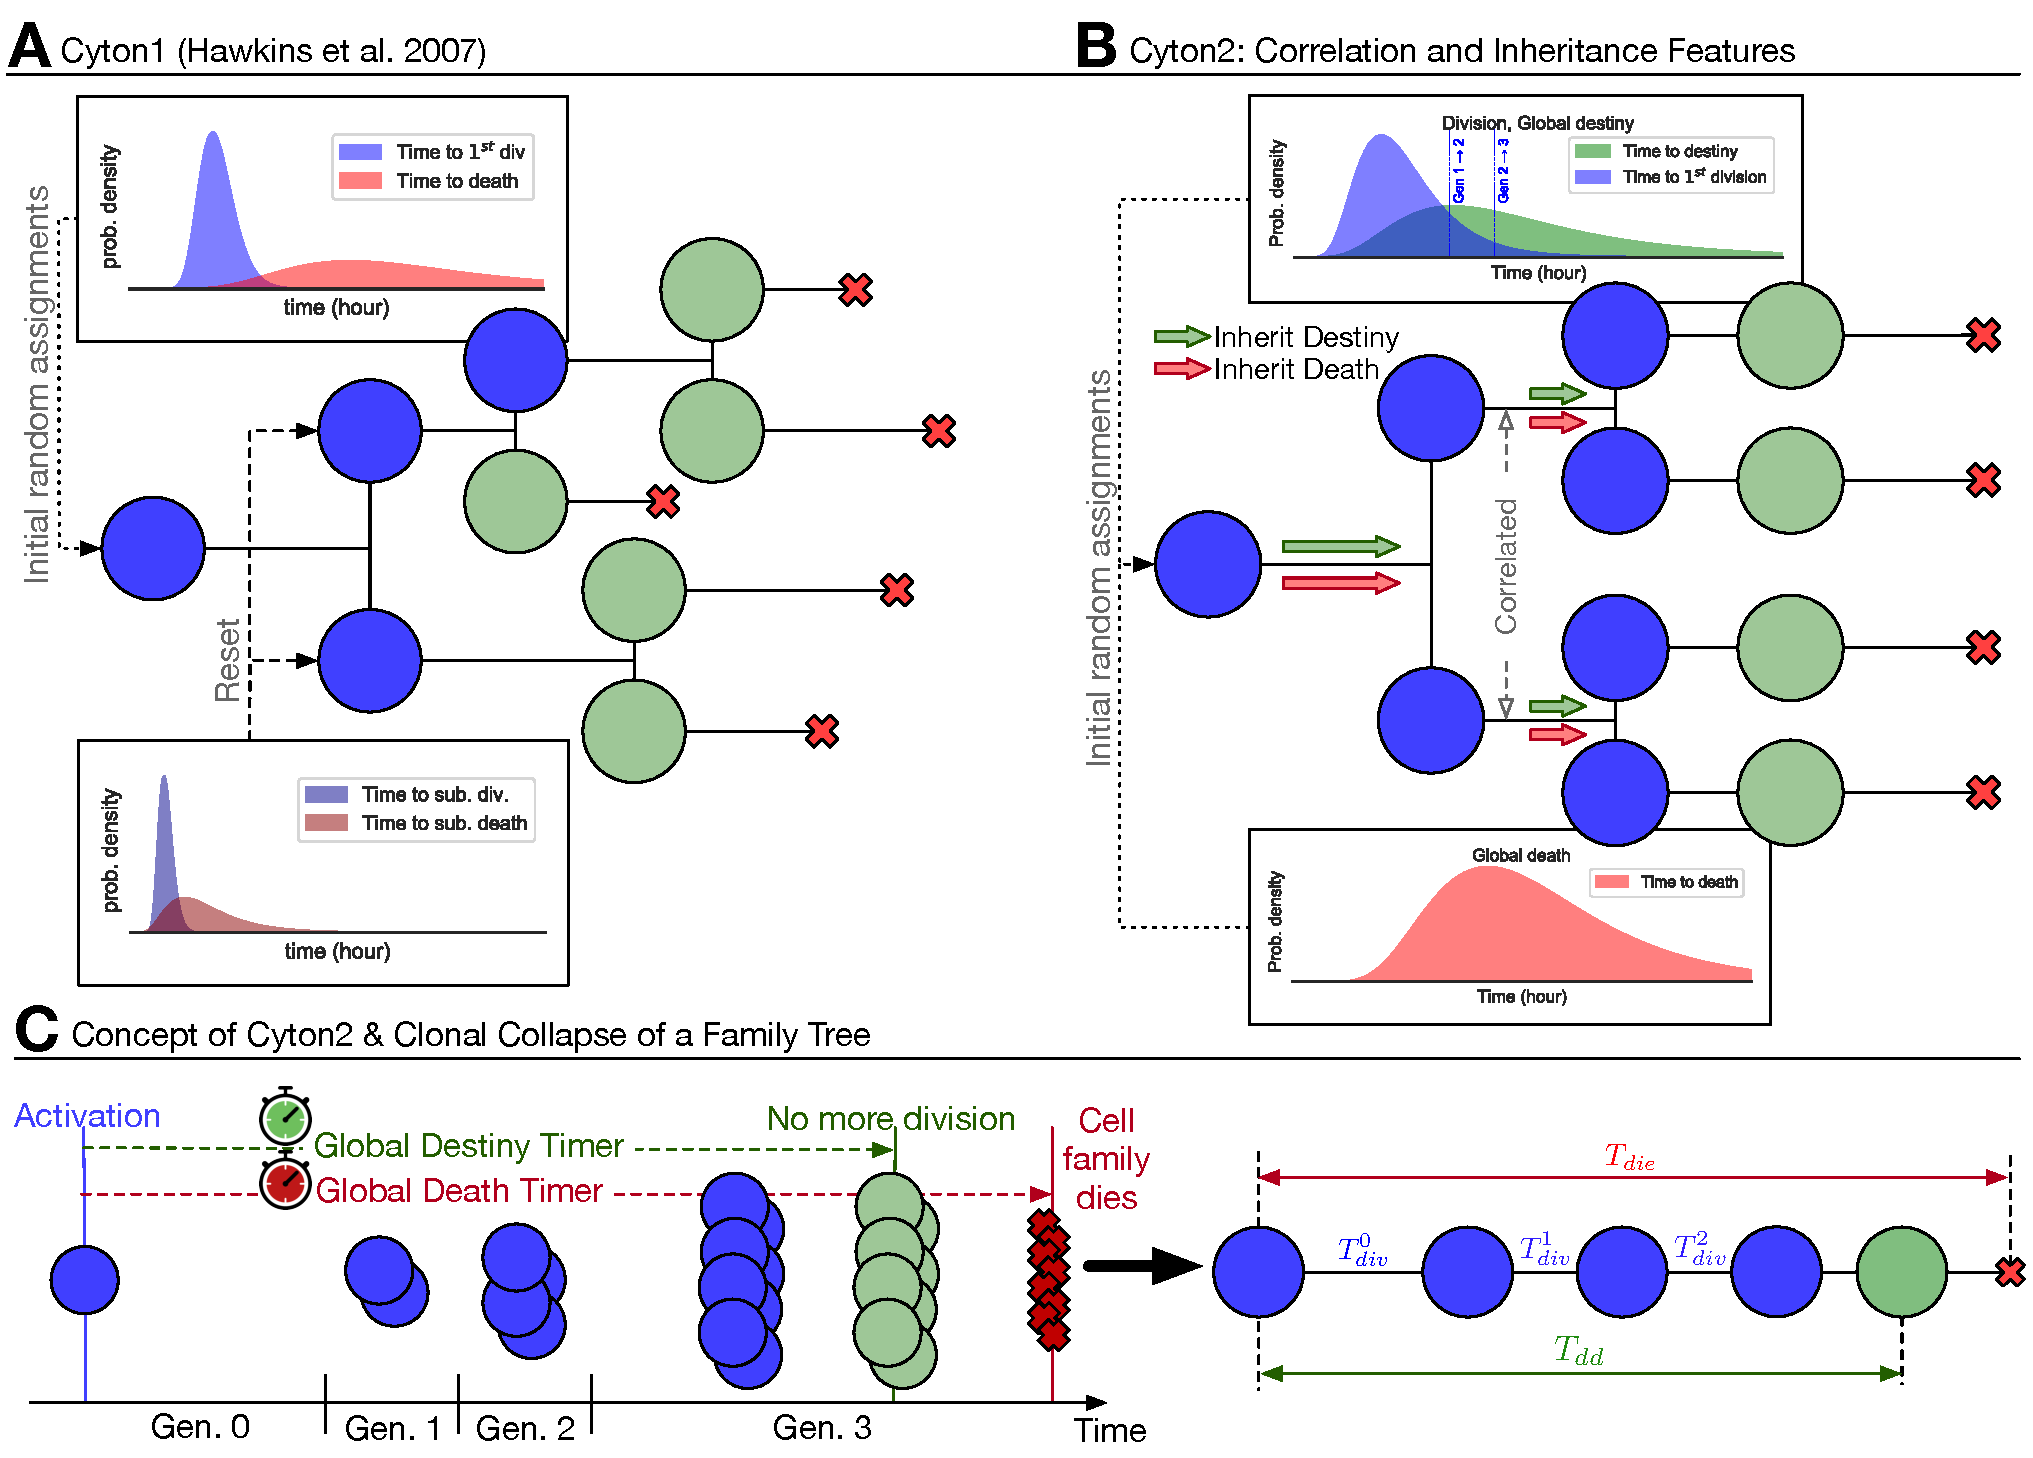
\includegraphics[scale=0.5]{figs/fig1.pdf}
    \caption{\textbf{Overview of the two Cyton models.} \textbf{(A)} The original Cyton model proposed in \cite{Hawkins.2007}. The times to divide and to death get reset every time the cell divides, then draw new random times for the offsprings. The cells cease to divide based on "counter" mechanism. \textbf{(B)} The new Cyton model that includes correlation of division times between siblings, and inheritance feature of time to death and to division destiny (time at which cells return to quiescent state). As opposed to the "counter" mechanism, the cells stop dividing at designated destiny time. \textbf{(C)} As a consequence of the correlation and inheritance, the family tree is highly concordant, depicted by the diagram. By exploiting this property, a family tree is summarised by substituting average values of the times at each generation. An example of clonally collapsed family tree and its key variables is shown.}
    \label{fig:model}
\end{figure}

% \linenumbers
While the original Cyton model captured and recreated immune cell population dynamics reasonably well (\cite{Hawkins.2007} and \cref{fig:model}A), recent findings in \cite{Heinzel.2016} impose two important modifications to the model. In the first, division destiny must be converted to a division-agnostic, timed mechanism, to replace the original generation counter. In the second, both destiny and death times should be programmed early after lymphocyte activation and applied globally within the developing family. Hence, time to destiny and time to die operate as a timer that is set once and the changing temporal register copied and transmitted through each division round \parencite{Heinzel.2016}. Consequently, the family tree of an activated lymphocyte is expected to be regular (\cref{fig:model}B) as, indeed, has been observed for both B and T cells \parencite{Hawkins.2009, Marchingo.2016}. Based on these findings, we formulate a new stochastic model of the lymphocyte response using sets of random variables (RVs) that correspond to global death timer, global destiny timer and division machinery (\cref{fig:model}C).

The first RV ($T_{die}$) represents the global death time for a family tree, where the founder cell is randomly assigned a time at which all progeny cells die. The second RV ($T_{dd}$) is the global destiny time after which no cells are allowed to progress to next generation and awaits only for death if $T_{dd} < T_{die}$ otherwise destiny event is censored by death. Lastly, the third RV ($T_{div}^k$) denotes for the time to division of cells at generation $k$. We define all three variables to span from the addition of stimulus, which is typically at $t=0$ in the experiment. However, the time to first division ($T_{div}^0$) and the subsequent division time ($M_k \coloneqq T_{div}^{k+1} - T_{div}^k$ for $k>0$) were reported to be two different quantities, for a lymphocyte typically takes longer time to complete its first division but, having done so, traverses subsequent division rounds at much faster and consistent rate \parencite{Gett.1998, Gett.2000}. We call the model Cyton2, a variant to the original Cyton model \parencite{Hawkins.2007} that extends to include not only correlation of division times between progeny cells but also inheritance of death and destiny times within a family.

Having defined the variables and operators of our new model, we first examined them for consistency with single cell data and with underlying assumptions. We were particularly interested in assessing evidence for the independent choice of times for division and death within individual cells, as assumed by Cyton and Cyton2 models \parencite{Gett.2000, Hawkins.2007}. We revisited two datasets for CpG-stimulated B cells published in \cite{Hawkins.2009} each consists of 108 clones (CpG3) and 88 clones (CpG4), respectively. Additionally, three CD8 T cell datasets were analysed: (i) with 1U, 3U and 10U of IL-2 seeded with 109, 90 and 163 clones, respectively; (ii) in combination of N4, aCD28 and IL-2 (Costim1); and, (iii) in combination of N4, aCD28 and IL-12 (Costim2). As an example, one B cell (CpG3) and T cell (IL-2) datasets are selected in this paper (see Supplementary \cref{supp_fig:raw_data} for all of raw data). For these analyses we transform family data by "collapsing" tree information, as shown in \cref{fig:model}C and described in Methods. This effectively linearises each family and allows features for the family to be examined and compared. Note that not all families were collapsible. For instance, if all members of a family were lost because they are indistinguishable to the nearby cells or survived until the end of movie, it is not possible to collapse as division and death time measurements are missing.

\begin{figure}[t]
    \centering
    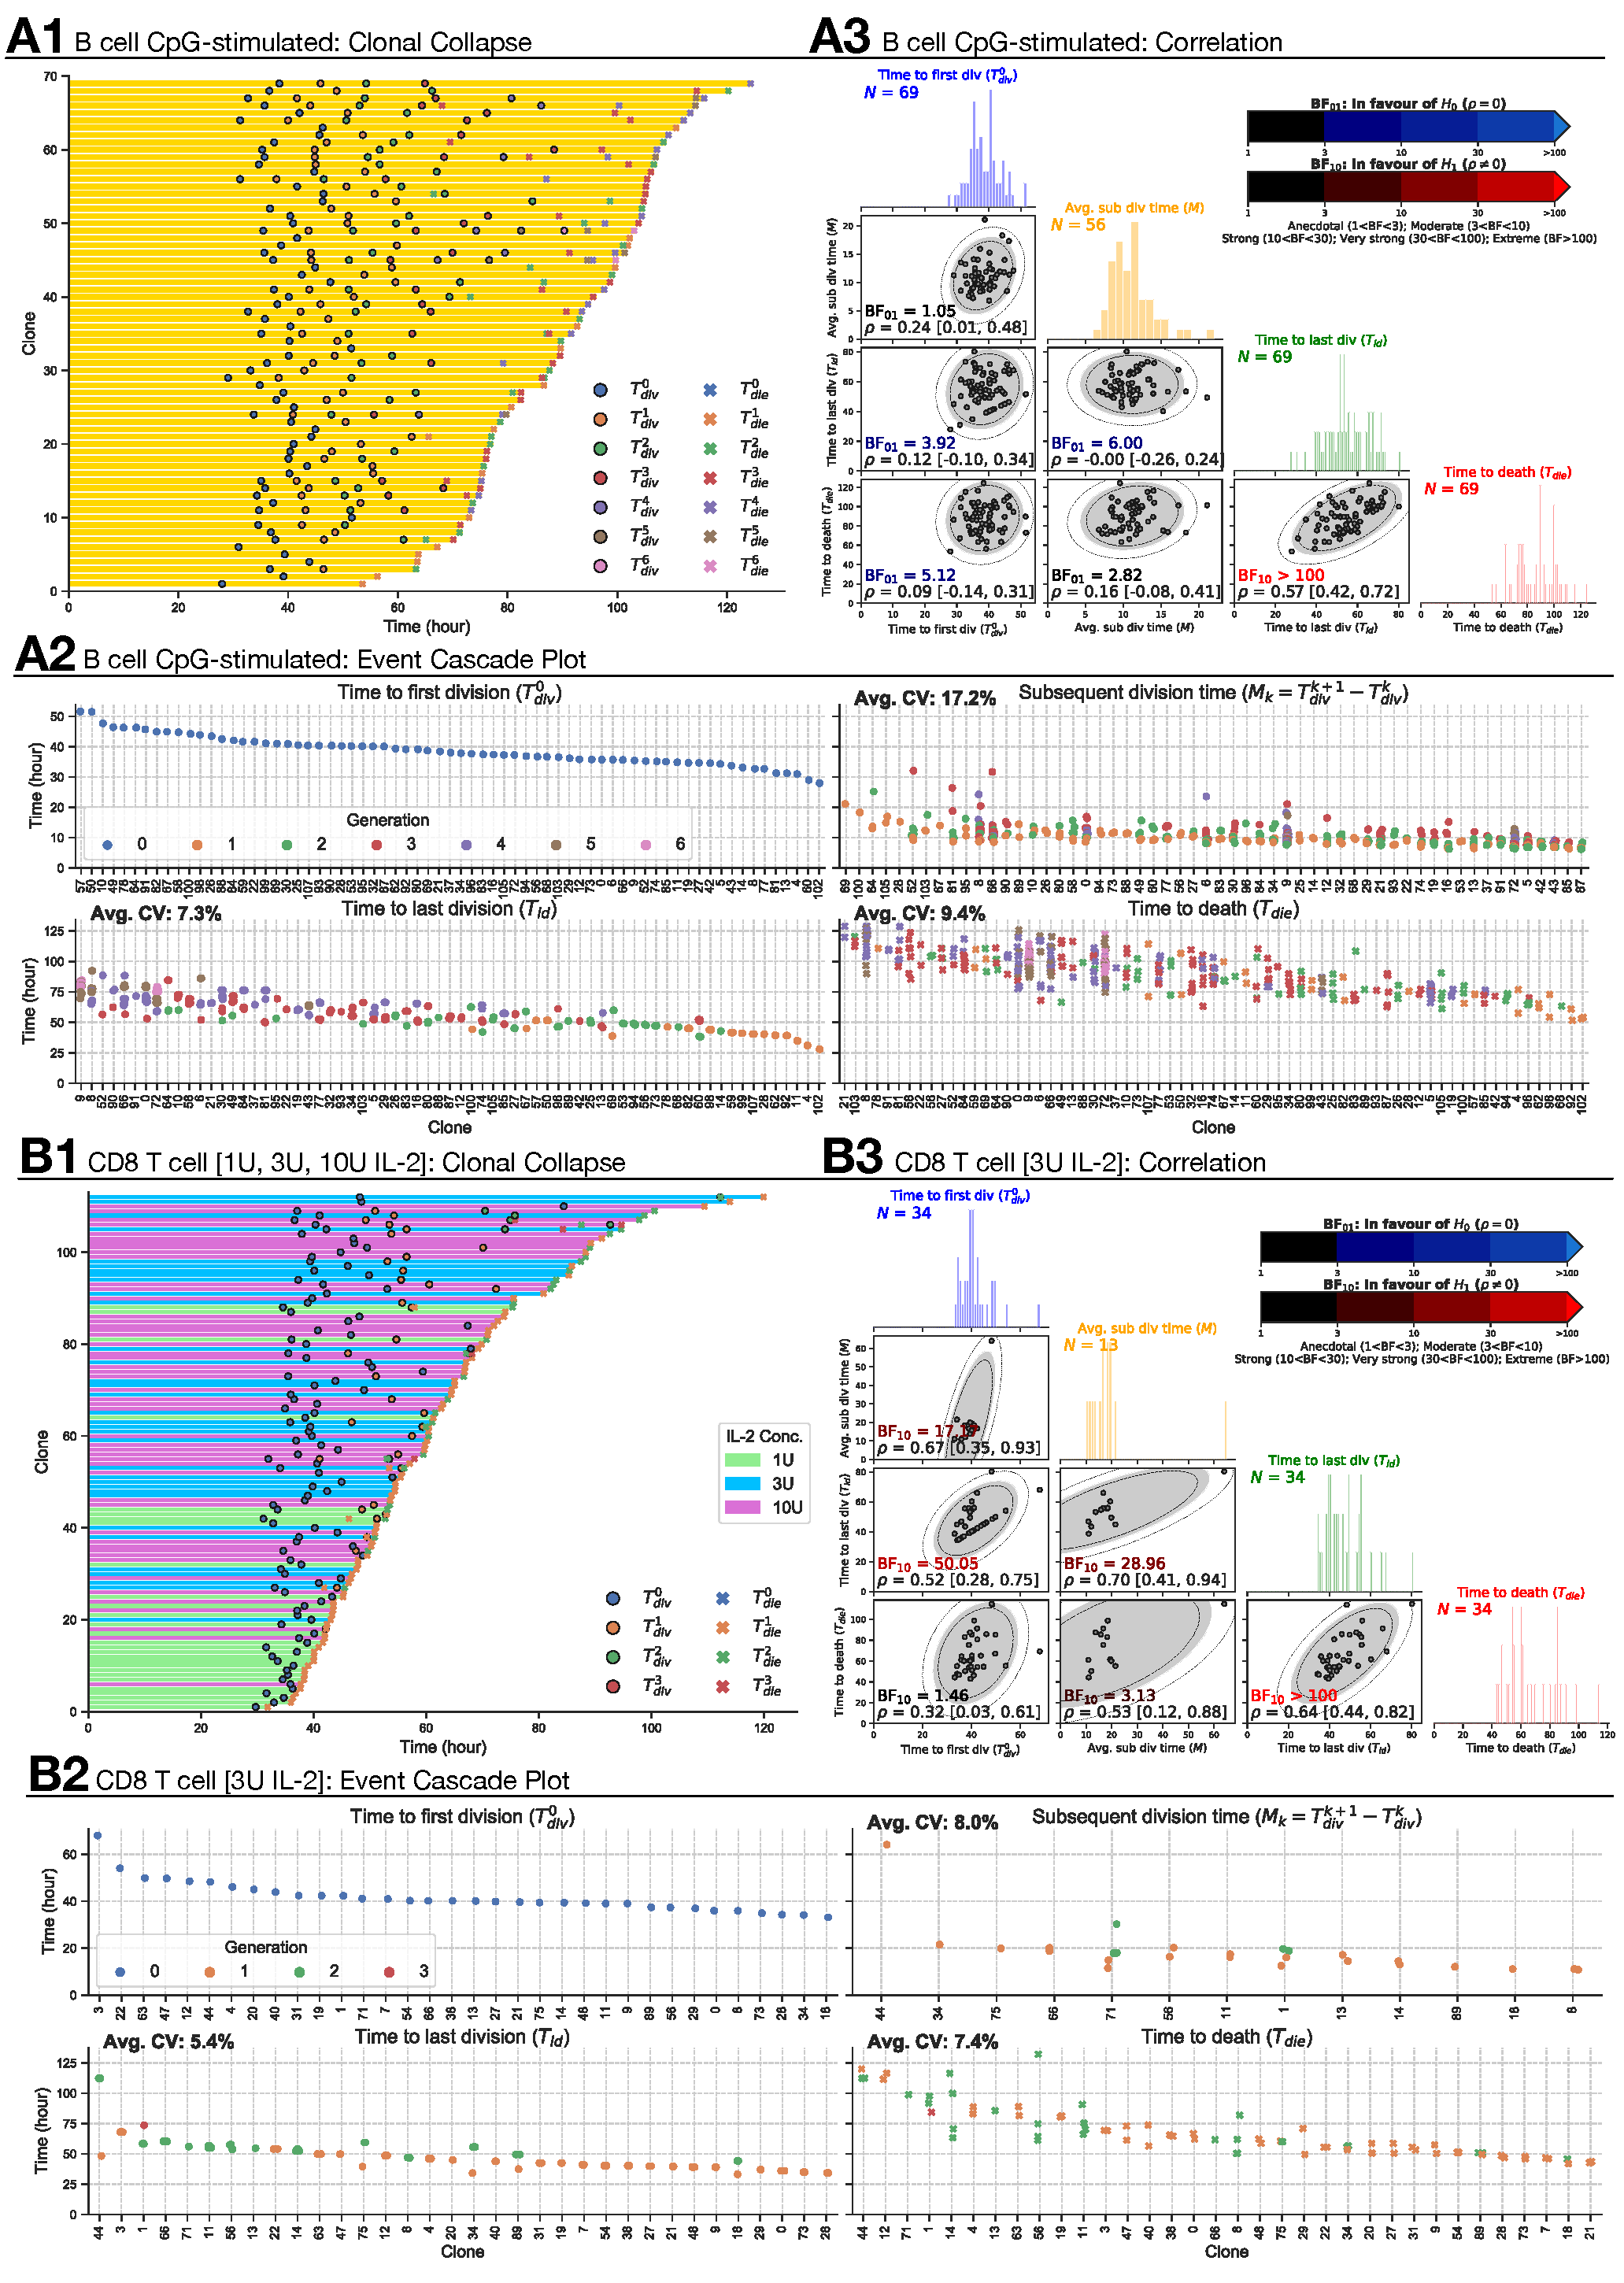
\includegraphics[scale=0.48]{figs/fig2.pdf}
    \caption{\textbf{Extracting times to fates from CpG-stimulated B cells and CD8 T cells in the presence of 1U, 3U or 10U IL-2.} \textbf{(A1, B1)} Clonally collapsed family trees from filtered data (lost cells not shown). \textbf{(A2, B2)} Measured times to events of the cells are shown and ordered by their average over all generations per clone. \textbf{(A3, B3)} Correlation coefficient ($\rho$) from bivariate normal distribution with 95\% credible interval is reported for each pair. 90\% (\dashed), 95\% (\colorbox{lightgray}{\makebox(12,3){\strut\textcolor{white}{}}}) and 99\% (\dotted) density regions are plotted over the data. Given null, H$_0$: $\rho = 0$, and alternative, H$_1$: $\rho \neq 0$, hypotheses, Bayes factor (BF$_{01} = 1/\mathrm{BF}_{10}$) is calculated. If the data is favoured under $H_0$, then it is BF$_{01}$ times more favoured than $H_1$ (\textit{blue-scale}), and vice versa (\textit{red-scale}). Distributions of the times are shown in the diagonal panels collated into $1h$ time intervals.}
    \label{fig:filming_data}
\end{figure}
\clearpage

\nolinenumbers
\subsection{Filming Data Supports Independent Operation of the Timers}
\label{sec:independence_of_timers}

\begingroup
\renewcommand{\arraystretch}{1.2}
\begin{table}[h]
    \resizebox{\textwidth}{!}{%
    \begin{tabular}{@{}clcccccc@{}}
    \toprule
    \multirow{2}{*}{\begin{tabular}[c]{@{}c@{}}Cell\\ Type\end{tabular}} &
      \multicolumn{1}{c}{\multirow{2}{*}{Stim.}} &
      \multicolumn{6}{c}{Bayes Factor (01/10) \& Correlation Coefficient ($\rho$ [CI])} \\
     &
      \multicolumn{1}{c}{} &
      ($T_{div}^0, M$) &
      ($T_{div}^0, T_{ld}$) &
      ($T_{div}^0, T_{die}$) &
      ($M, T_{ld}$) &
      ($M, T_{die}$) &
      ($T_{ld}, T_{die}$) \\ \cmidrule(l){1-2} \cmidrule(l){3-3} \cmidrule(l){4-4} \cmidrule(l){5-5} \cmidrule(l){6-6} \cmidrule(l){7-7} \cmidrule(l){8-8} 
    B &
      CpG &
      \begin{tabular}[c]{@{}c@{}}\textcolor{bf01_1}{1.05 (01)}\\ 0.24 {[}0.01, 0.48{]}\end{tabular} &
      \begin{tabular}[c]{@{}c@{}}\textcolor{bf01_2}{3.92 (01)}\\ 0.12 {[}-0.10, 0.34{]}\end{tabular} &
      \begin{tabular}[c]{@{}c@{}}\textcolor{bf01_2}{5.12 (01)}\\ 0.09 {[}-0.14, 0.31{]}\end{tabular} &
      \begin{tabular}[c]{@{}c@{}}\textcolor{bf01_2}{6.00 (01)}\\ 0.0 {[}-0.26, 0.24{]}\end{tabular} &
      \begin{tabular}[c]{@{}c@{}}\textcolor{bf01_1}{2.82 (01)}\\ 0.16 {[}-0.08, 0.41{]}\end{tabular} &
      \begin{tabular}[c]{@{}c@{}}\textcolor{bf10_5}{\textgreater{}100 (10)}\\ 0.57 {[}0.42, 0.72{]}\end{tabular} \\ \midrule
    \multirow{3}{*}{\begin{tabular}[c]{@{}c@{}}CD8 T\\ (+IL2)\end{tabular}} &
      1U &
      \begin{tabular}[c]{@{}c@{}}\textcolor{bf01_1}{1.70 (01)}\\ -0.01 {[}-0.87, 0.85{]}\end{tabular} &
      \begin{tabular}[c]{@{}c@{}}\textcolor{bf10_4}{39.09 (10)}\\ 0.55 {[}0.29, 0.79{]}\end{tabular} &
      \begin{tabular}[c]{@{}c@{}}\textcolor{bf01_1}{2.53 (01)}\\ 0.19 {[}-0.16, 0.53{]}\end{tabular} &
      \begin{tabular}[c]{@{}c@{}}\textcolor{bf01_1}{1.53 (01)}\\ -0.15 {[}-0.97, 0.70{]}\end{tabular} &
      \begin{tabular}[c]{@{}c@{}}\textcolor{bf01_1}{1.43 (01)}\\ 0.20 {[}-0.67, 0.98{]}\end{tabular} &
      \begin{tabular}[c]{@{}c@{}}\textcolor{bf10_5}{\textgreater{}100 (10)}\\ 0.59 {[}0.36, 0.81{]}\end{tabular} \\
     &
      3U &
      \begin{tabular}[c]{@{}c@{}}\textcolor{bf10_3}{17.17 (10)}\\ 0.67 {[}0.35, 0.93{]}\end{tabular} &
      \begin{tabular}[c]{@{}c@{}}\textcolor{bf10_4}{50.05 (10)}\\ 0.52 {[}0.28, 0.75{]}\end{tabular} &
      \begin{tabular}[c]{@{}c@{}}\textcolor{bf10_1}{1.46 (10)}\\ 0.32 {[}0.03, 0.61{]}\end{tabular} &
      \begin{tabular}[c]{@{}c@{}}\textcolor{bf10_3}{28.96 (10)}\\ 0.70 {[}0.41, 0.94{]}\end{tabular} &
      \begin{tabular}[c]{@{}c@{}}\textcolor{bf10_2}{3.13 (10)}\\ 0.53 {[}0.12, 0.88{]}\end{tabular} &
      \begin{tabular}[c]{@{}c@{}}\textcolor{bf10_5}{\textgreater{}100 (10)}\\ 0.64 {[}0.44, 0.82{]}\end{tabular} \\
     &
      10U &
      \begin{tabular}[c]{@{}c@{}}\textcolor{bf10_2}{7.55 (10)}\\ 0.57 {[}0.23, 0.87{]}\end{tabular} &
      \begin{tabular}[c]{@{}c@{}}\textcolor{bf10_5}{\textgreater{}100 (10)}\\ 0.58 {[}0.40, 0.75{]}\end{tabular} &
      \begin{tabular}[c]{@{}c@{}}\textcolor{bf10_3}{15.39 (10)}\\ 0.40 {[}0.18, 0.62{]}\end{tabular} &
      \begin{tabular}[c]{@{}c@{}}\textcolor{bf10_5}{\textgreater{}100 (10)}\\ 0.76 {[}0.55, 0.94{]}\end{tabular} &
      \begin{tabular}[c]{@{}c@{}}\textcolor{bf10_1}{1.56 (10)}\\ 0.42 {[}0.02, 0.79{]}\end{tabular} &
      \begin{tabular}[c]{@{}c@{}}\textcolor{bf10_5}{\textgreater{}100 (10)}\\ 0.63 {[}0.46, 0.78{]}\end{tabular} \\ 
      \bottomrule
    \end{tabular}%
    }
    \caption{\textbf{Test correlation of every pair of times to fates.} The correlation coefficient calculated from a bivariate normal distribution with its 95\% credible interval is shown for CpG-stimulated B cell and CD8 T cell in the presence of 1U, 3U or 10U of IL-2. The same Bayes factor interpretation criterion is used as shown in \cref{fig:filming_data}.}
    \label{tab:independence}
\end{table}
\endgroup

% \linenumbers
\noindent
In \cref{fig:filming_data}A1 and B1, we plotted clonally collapsed family trees of filtered clones as a single representative time line stacked vertically for CpG-stimulated B cells (CpG3: 69 clones) and CD8 T cells in the presence of 1U (28 clones), 3U (34 clones) and 10U (50 clones) of IL-2. The average times to division and to death are marked at each generation (see Methods). The key Cyton2 variables are shown in the cascade plot for all cells in a family with the exception of time to division destiny ($T_{dd}$). Here, $T_{dd}$ cannot be identified and was replaced with time to last division ($T_{ld}$) as a proxy measure (\cref{fig:filming_data}A2, B2; \cref{supp_fig:costims} for Costim1 and Costim2). Given the distributions of these measurements, we asked the spreads of subsequent division time ($M_k$), time to last division and time to death ($T_{die}$) within a clone to see if the cells reached fates synchronously as reported in \cite{Hawkins.2009, Marchingo.2016, Mitchell.2018}. To quantify this, we calculated coefficient of variation (CV) per clone, and then took the average of CVs for each variables. In the order of $M_k$, $T_{ld}$ and $T_{die}$, we identified 17.2\%, 7.3\% and 9.4\% of average CVs for B cells and 8\%, 5.4\% and 7.4\% for T cells. Similar results were shown for a repeat of B cell (73 clones) and CD8 T cells with 1U and 10U of IL-2 (\cref{supp_fig:repeats}). This signifies low variation around the mean times to fates and is consistent with the reported synchronous behaviour of the cells. Given this conclusion, we turned our attention to the question of the independence of the variables operating at the clone level. Here, for statistical purpose, we extracted time to first division, average subsequent division time ($M$), average time to last division and average time to death as four key variables per clone. For every pairs of these variables, the correlation coefficient ($\rho$) and its 95\% credible interval were determined from Bayesian inference. Moreover, Bayes factor (BF) for two competing hypotheses (H$_0: \rho = 0$ and H$_1: \rho \neq 0$) were calculated (see Methods) (\cref{fig:filming_data}A3, B3). The estimates of these quantities are shown in \cref{tab:independence} (see Supplementary \cref{tab:costim_independence} for Costim1 and Costim2). With the exception of ($T_{ld}, T_{die}$) pair for all datasets, CpG-stimulated B cells are consistent with the independence assumption of the operation of the times. However, we discovered 10 pairs of variables were reported with BF$_{10}>10$ for T cells, indicating strong evidence towards correlation. This result at face value appears to violate the independence assumption. However, as we noted previously, censorship of fates can lead to faux correlations between independent outcomes \parencite{Duffy.2012, Duffy.2012j67}. We explore this possibility in the following section by generating large number of Cyton2 trees \textit{in sillico} under the independence assumption.

\nolinenumbers
\subsection{Censorship of the Timers}
\label{sec:censorship}
\begin{figure}[t]
    \centering
    \includegraphics[scale=0.49]{figs/fig3.pdf}
    \caption{\textbf{Simulation under the independence assumption.} $10^6$ families were simulated via Cyton2-like ABM given fitted lognormal distributions of $T_{div}^0$, $M$, $T_{ld}$, $T_{die}$ from respective data. \textbf{(A1)} Three example families of ABM realisation for CpG-stimulated B cells: dividing (\textcolor{blue}{\full}) and dying (\textcolor{red}{\full}) states. The realisations of $T_{div}^0$ (\textcolor{blue}{$\bullet$}), $M$ ($m$), $T_{ld}$ (\textcolor{ForestGreen}{$\bullet$}), $T_{dd}$ (\textcolor{ForestGreen}{$\star$}) and $T_{die}$ (\textcolor{red}{$\times$}) are annotated on a clonally collapsed line. As features of inheritance and correlation, the cells double in number synchronously whenever division occurs, and likewise, all cells reach destiny and death at the same time. (\textbf{A2, B1-3}) Sampled true (\textcolor{abm_true}{$\bullet$}) times to fates for all simulated families and their corresponding observable (\textcolor{abm_obs}{$\bullet$}) values are shown in pairs along with the data points (\textcolor{abm_data}{$\bullet$}). The observable and unobservable regions are separated by upper and lower sections of $y=x$ line (\dashed), respectively. The Bayes factors are reported for the true and observable pairs.}
    \label{fig:ABM_simulation}
\end{figure}

\begingroup
\renewcommand{\arraystretch}{1.5}
\begin{table}[h]
    \resizebox{\textwidth}{!}{%
    \begin{tabular}{@{}clcccccccccccc@{}}
    \toprule
    \multirow{3}{*}{\begin{tabular}[c]{@{}c@{}}Cell\\ Type\end{tabular}} &
      \multicolumn{1}{c}{\multirow{3}{*}{Stim.}} &
      \multicolumn{12}{c}{Bayes Factor (01/10) of True and Observable values from $10^6$ simulated families} \\
      & \multicolumn{1}{c}{} &
      \multicolumn{2}{c}{($T_{div}^0, M$)} &
      \multicolumn{2}{c}{($T_{div}^0, T_{ld}$)} &
      \multicolumn{2}{c}{($T_{div}^0, T_{die}$)} &
      \multicolumn{2}{c}{($M, T_{ld}$)} &
      \multicolumn{2}{c}{($M, T_{die}$)} &
      \multicolumn{2}{c}{($T_{ld}, T_{die}$)} \\ 
      & \multicolumn{1}{c}{} &
      True & Obs. &
      True & Obs. &
      True & Obs. &
      True & Obs. &
      True & Obs. &
      True & Obs. \\
      \cmidrule(l){1-2} \cmidrule(l){3-4} \cmidrule(l){5-6} \cmidrule(l){7-8} \cmidrule(l){9-10} \cmidrule(l){11-12} \cmidrule(l){13-14} 
      B & CpG &
      \begin{tabular}[c]{@{}c@{}}\textcolor{bf01_5}{\textgreater{}100 (01)}\end{tabular} &
      \begin{tabular}[c]{@{}c@{}}\textcolor{bf10_5}{\textgreater{}100 (10)}\end{tabular} &
      \begin{tabular}[c]{@{}c@{}}\textcolor{bf01_5}{\textgreater{}100 (01)}\end{tabular} &
      \begin{tabular}[c]{@{}c@{}}\textcolor{bf10_5}{\textgreater{}100 (10)}\end{tabular} &
      \begin{tabular}[c]{@{}c@{}}\textcolor{bf01_5}{\textgreater{}100 (01)}\end{tabular} &
      \begin{tabular}[c]{@{}c@{}}\textcolor{bf01_5}{\textgreater{}100 (01)}\end{tabular} &
      \begin{tabular}[c]{@{}c@{}}\textcolor{bf01_5}{\textgreater{}100 (01)}\end{tabular} &
      \begin{tabular}[c]{@{}c@{}}\textcolor{bf10_5}{\textgreater{}100 (10)}\end{tabular} &
      \begin{tabular}[c]{@{}c@{}}\textcolor{bf01_5}{\textgreater{}100 (01)}\end{tabular} &
      \begin{tabular}[c]{@{}c@{}}\textcolor{bf01_2}{4.32 (01)}\end{tabular} &
      \begin{tabular}[c]{@{}c@{}}\textcolor{bf01_5}{\textgreater{}100 (01)}\end{tabular} &
      \begin{tabular}[c]{@{}c@{}}\textcolor{bf10_5}{\textgreater{}100 (10)}\end{tabular} \\ \midrule
 
    \multirow{3}{*}{\begin{tabular}[c]{@{}c@{}}CD8 T\\ (+IL2)\end{tabular}} & 1U &
    \begin{tabular}[c]{@{}c@{}}\textcolor{bf01_5}{\textgreater{}100 (01)}\end{tabular} &
      \begin{tabular}[c]{@{}c@{}}\textcolor{bf10_5}{\textgreater{}100 (10)}\end{tabular} &
      \begin{tabular}[c]{@{}c@{}}\textcolor{bf01_5}{\textgreater{}100 (01)}\end{tabular} &
      \begin{tabular}[c]{@{}c@{}}\textcolor{bf10_5}{\textgreater{}100 (10)}\end{tabular} &
      \begin{tabular}[c]{@{}c@{}}\textcolor{bf01_5}{\textgreater{}100 (01)}\end{tabular} &
      \begin{tabular}[c]{@{}c@{}}\textcolor{bf10_5}{\textgreater{}100 (10)}\end{tabular} &
      \begin{tabular}[c]{@{}c@{}}\textcolor{bf01_5}{\textgreater{}100 (01)}\end{tabular} &
      \begin{tabular}[c]{@{}c@{}}\textcolor{bf10_5}{\textgreater{}100 (10)}\end{tabular} &
      \begin{tabular}[c]{@{}c@{}}\textcolor{bf01_5}{\textgreater{}100 (01)}\end{tabular} &
      \begin{tabular}[c]{@{}c@{}}\textcolor{bf10_5}{\textgreater{}100 (10)}\end{tabular} &
      \begin{tabular}[c]{@{}c@{}}\textcolor{bf01_5}{\textgreater{}100 (01)}\end{tabular} &
      \begin{tabular}[c]{@{}c@{}}\textcolor{bf10_5}{\textgreater{}100 (10)}\end{tabular} \\
     & 3U &
     \begin{tabular}[c]{@{}c@{}}\textcolor{bf01_5}{\textgreater{}100 (01)}\end{tabular} &
     \begin{tabular}[c]{@{}c@{}}\textcolor{bf10_5}{\textgreater{}100 (10)}\end{tabular} &
     \begin{tabular}[c]{@{}c@{}}\textcolor{bf01_5}{\textgreater{}100 (01)}\end{tabular} &
     \begin{tabular}[c]{@{}c@{}}\textcolor{bf10_5}{\textgreater{}100 (10)}\end{tabular} &
     \begin{tabular}[c]{@{}c@{}}\textcolor{bf01_5}{\textgreater{}100 (01)}\end{tabular} &
     \begin{tabular}[c]{@{}c@{}}\textcolor{bf10_5}{\textgreater{}100 (10)}\end{tabular} &
     \begin{tabular}[c]{@{}c@{}}\textcolor{bf01_5}{\textgreater{}100 (01)}\end{tabular} &
     \begin{tabular}[c]{@{}c@{}}\textcolor{bf10_5}{\textgreater{}100 (10)}\end{tabular} &
     \begin{tabular}[c]{@{}c@{}}\textcolor{bf01_5}{\textgreater{}100 (01)}\end{tabular} &
     \begin{tabular}[c]{@{}c@{}}\textcolor{bf10_5}{\textgreater{}100 (10)}\end{tabular} &
     \begin{tabular}[c]{@{}c@{}}\textcolor{bf01_5}{\textgreater{}100 (01)}\end{tabular} &
     \begin{tabular}[c]{@{}c@{}}\textcolor{bf10_5}{\textgreater{}100 (10)}\end{tabular} \\
     & 10U &
     \begin{tabular}[c]{@{}c@{}}\textcolor{bf01_5}{\textgreater{}100 (01)}\end{tabular} &
     \begin{tabular}[c]{@{}c@{}}\textcolor{bf10_5}{\textgreater{}100 (10)}\end{tabular} &
     \begin{tabular}[c]{@{}c@{}}\textcolor{bf01_5}{\textgreater{}100 (01)}\end{tabular} &
     \begin{tabular}[c]{@{}c@{}}\textcolor{bf10_5}{\textgreater{}100 (10)}\end{tabular} &
     \begin{tabular}[c]{@{}c@{}}\textcolor{bf01_5}{\textgreater{}100 (01)}\end{tabular} &
     \begin{tabular}[c]{@{}c@{}}\textcolor{bf10_5}{\textgreater{}100 (10)}\end{tabular} &
     \begin{tabular}[c]{@{}c@{}}\textcolor{bf01_5}{\textgreater{}100 (01)}\end{tabular} &
     \begin{tabular}[c]{@{}c@{}}\textcolor{bf10_5}{\textgreater{}100 (10)}\end{tabular} &
     \begin{tabular}[c]{@{}c@{}}\textcolor{bf01_5}{\textgreater{}100 (01)}\end{tabular} &
     \begin{tabular}[c]{@{}c@{}}\textcolor{bf10_5}{\textgreater{}100 (10)}\end{tabular} &
     \begin{tabular}[c]{@{}c@{}}\textcolor{bf01_5}{\textgreater{}100 (01)}\end{tabular} &
     \begin{tabular}[c]{@{}c@{}}\textcolor{bf10_5}{\textgreater{}100 (10)}\end{tabular} \\
      \bottomrule
    \end{tabular}%
    }
    \caption{\textbf{Test correlation for the simulated trees.} The Bayes factors were calculated same way as the \cref{tab:data}. \textit{Blue} indicates more probable under the null hypothesis ($\rho=0$) and \textit{red} indicates more probably under the alternative hypothesis ($\rho \neq 0$).}
    \label{tab:independence_simulation}
\end{table}
\endgroup

% \linenumbers
\noindent
In \cref{sec:independence_of_timers}, CpG-stimulated B cells were reported to be more probable under no correlation for most of the variable pairs while CD8 T cells had mixed results. The key difference between two datasets is the depth of the trees: many of B cells had divided as many as six times whereas T cells had divided at most three times (\cref{fig:filming_data}A2, B2). This suggests that many of variables are rendered unobserved or even censored for T cells. If the variables are truly independent of each other, any order of times to fates could had been assigned to each family. For example, if $T_{die} < \min(T_{div}, T_{dd})$, then the time to first division and destiny would be censored by the death event. For this reason, the timers may have operated independently, but the realisation of those timers are appeared to be neccessarily correlated.

We simulated Cyton2-like process via agent-based model (see Methods) to recapitulate the filming data. Under the assumption that $T_{ld} = T_{dd}$, each of variables was randomly sampled from respective fitted lognormal distribution from the data (see \cref{sec:distribution_class}). Both observable and true assigned values are plotted in \cref{fig:ABM_simulation}A2 for B cells and \cref{fig:ABM_simulation}B1-3 for T cells. It clearly shows that T cells have more censorship than that of B cells, which is directly translated from significant overlapping of the distributions. The Bayes factor under the same hypotheses used in \cref{sec:independence_of_timers} showed that the true values are more probable under the null hypothesis (H$_0: \rho=0$) as expected while it favours the alternative hypothesis (H$_1: \rho \neq 0$) for the observable values most of times (\cref{tab:independence_simulation}). In fact, all of the pairs for the observable values were reported strongly correlated for T cells as a result of high degree censorship. Interestingly, ($T_{div}^0, M$), ($T_{div}^0, T_{ld}$), ($M, T_{ld}$) and ($T_{ld}, T_{die}$) pairs from B cells were reported correlated for larger number of clones, otherwise the rest of pairs exhibited lack of correlation as reported directly from the B cell data. Thus, we illustrate and confirm that timers may well be operating independent to each other but the resulting outcome can appear correlated. We conclude from the simulation that correlation is not an inherent feature of the competing timers but results as a consequence of the censorship. Thus, minimally, the data can be interpreted as consistent with the independence assumption.

\nolinenumbers
\subsection{Using Filming Data to Obtain Best Distribution Class for the Timers}
\label{sec:distribution_class}
\begin{figure}[t]
    \centering
    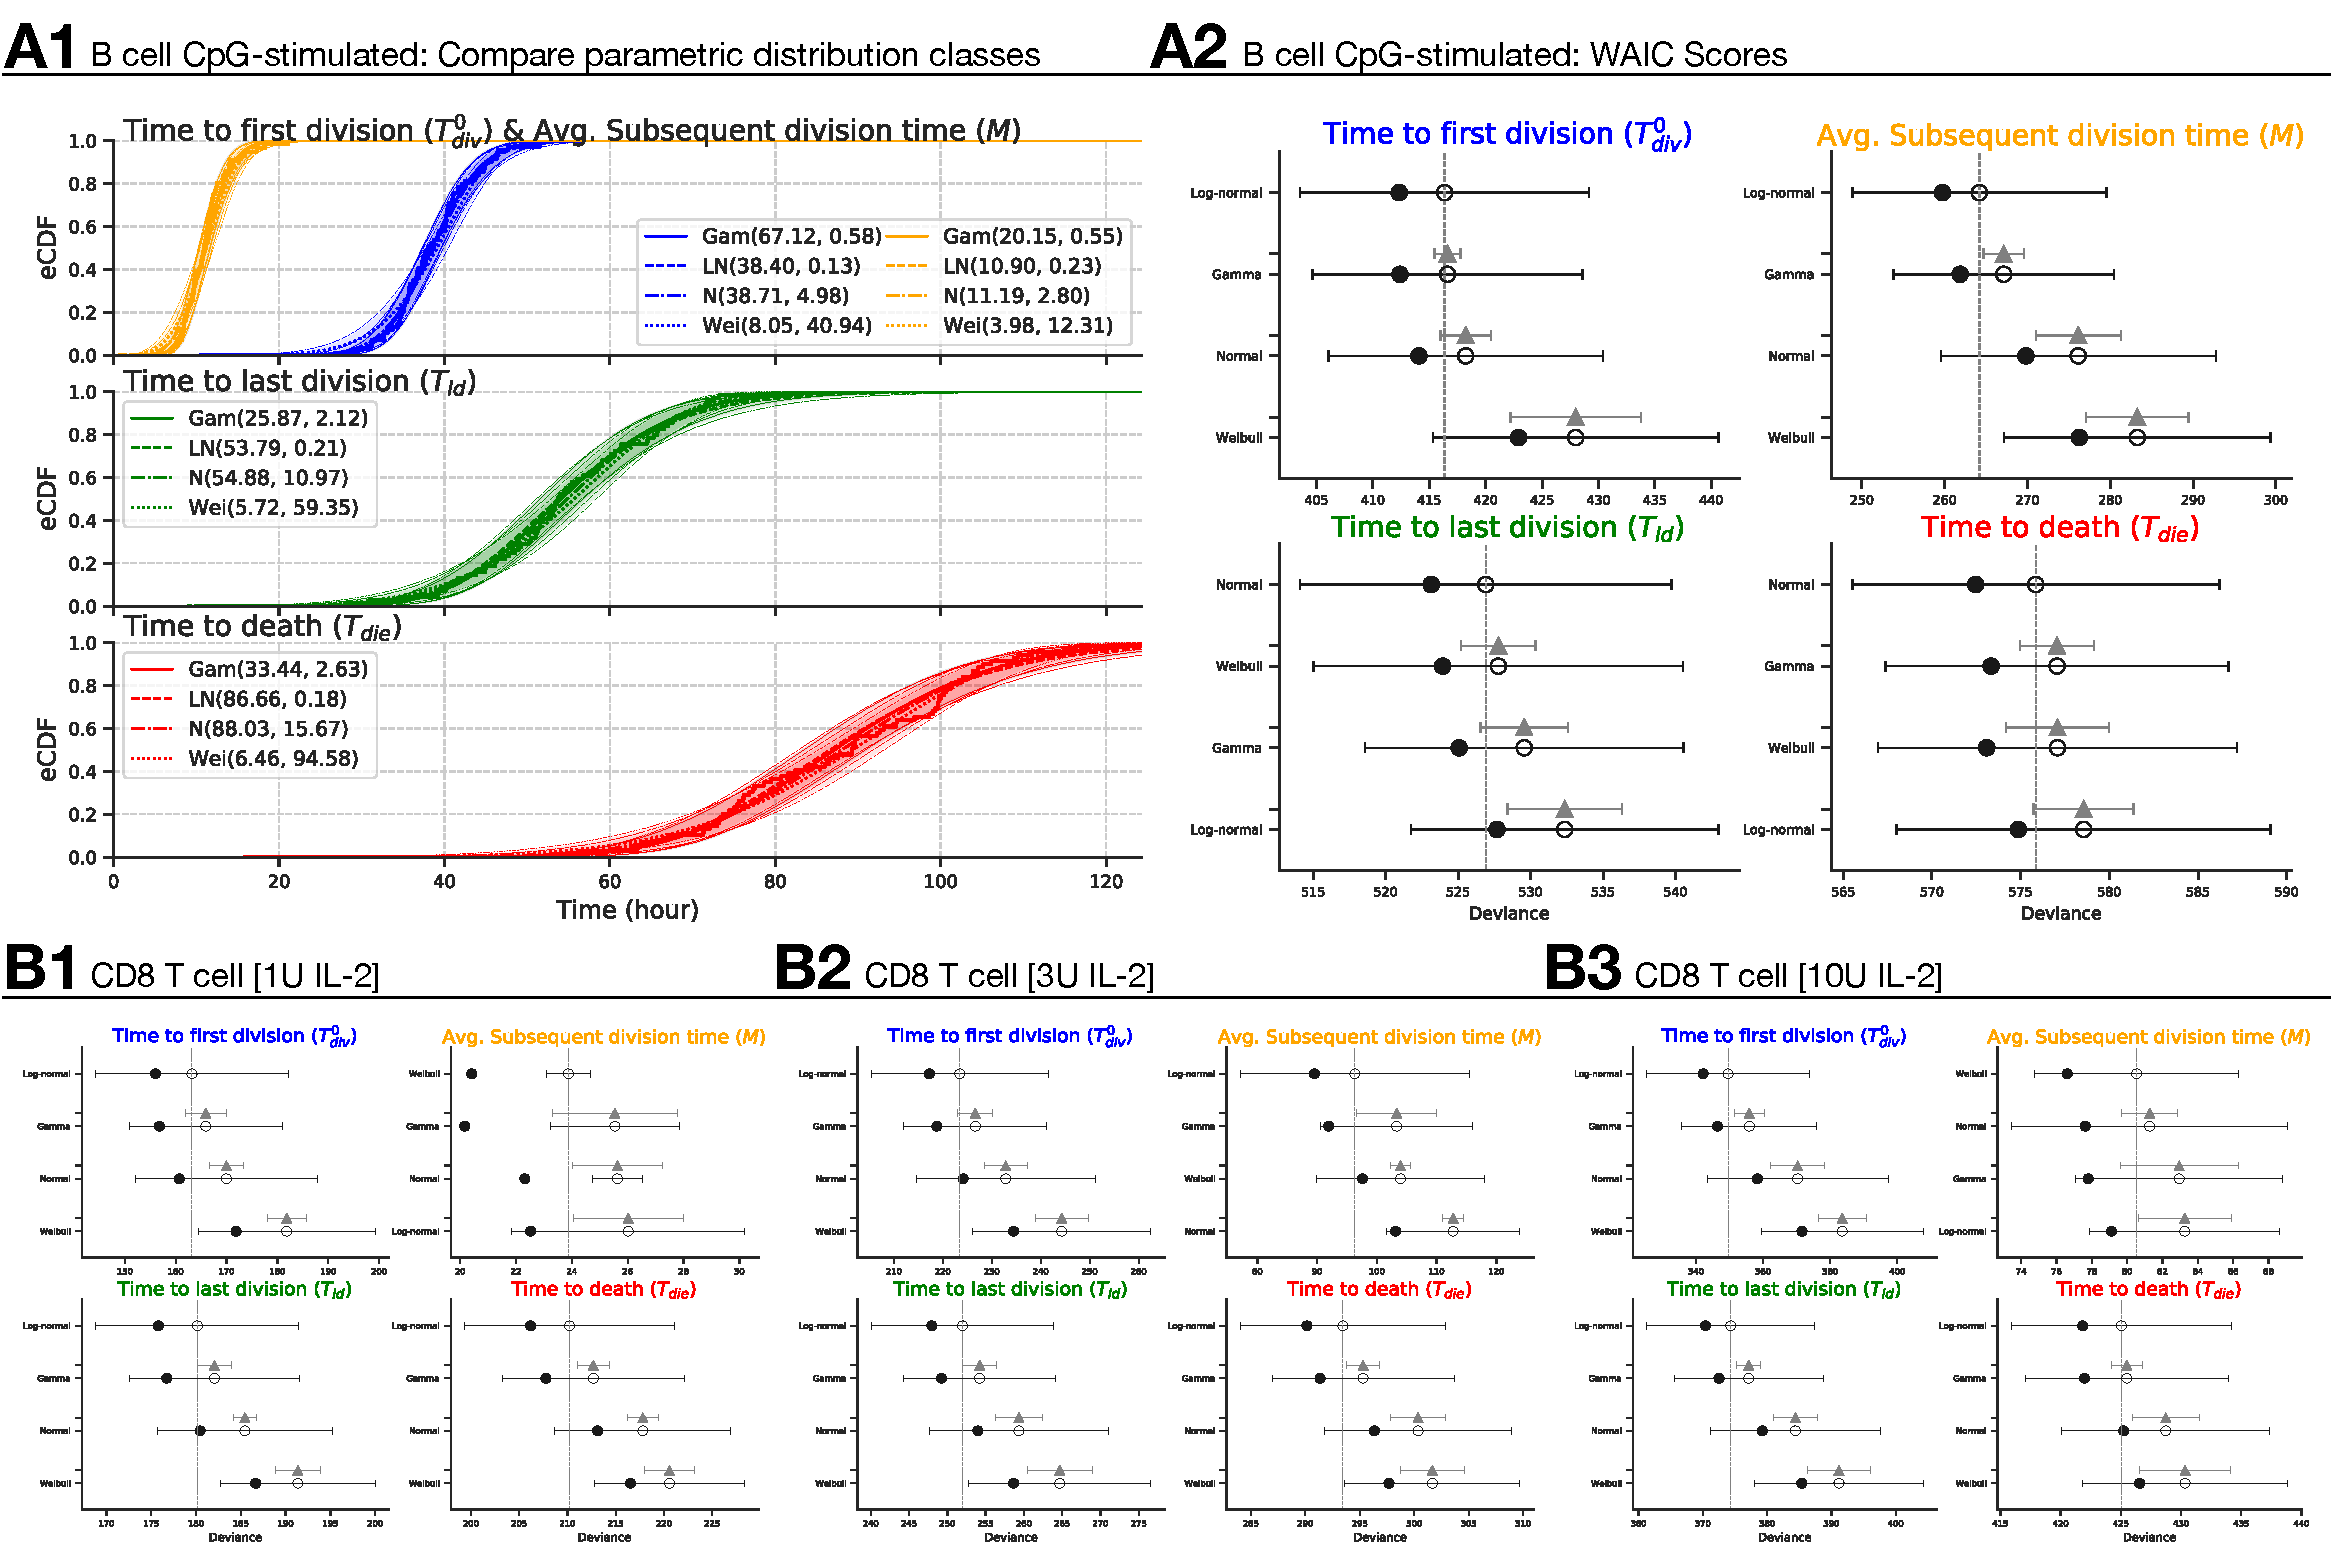
\includegraphics[scale=0.45]{figs/fig4.pdf}
    \caption{\textbf{Best parametric distribution class.} \textbf{(A1)} Empirical CDF of the measured times are overlaid with CDFs of Gamma, Lognormal, Normal and Weibull distributions. 95\% confidence bands are plotted by randomly drawing $10^4$ samples from respective posterior distributions. \textbf{(A2, B1-3)} The in-sample deviance ($\bullet$), and WAIC scores ($\circ$) with 1 standard deviation error bar are shown. The y-axis is sorted from lowest (\textit{top-row}) to highest (\textit{bottom-row}) WAIC score. The lower WAIC score indicates better descriptor of the data. Except the top-ranked one, the value of the difference of WAIC (\textcolor{gray}{$\blacktriangle$}) between a candidate and the top-ranked are shown with 1 standard error of the difference.}
    \label{fig:best_distribution}
\end{figure}
% \linenumbers
Identifying a parametric distribution class for the variables is another crucial components in the development of the model. In the literature, the probability distributions governing the times to first division and to death were reported to be well approximated by a right-skewed distribution such as Lognormal, Weibull, Gamma or Beta \parencite{Hawkins.2009}. In particular, the time to first division is known to be better described by a Lognormal than other skew distributions whereas Gamma or Weibull distributions can be used to approximate the time to death distribution \parencite{Hawkins.2007}. However, the distribution of the time to division destiny is still unknown. Although the "true" distribution of the timers may not be possible to obtain, we can infer a better descriptor by employing Bayesian model selection criteria (see Methods).

In \cref{fig:best_distribution}A, we plotted empirical cumulative distribution function (eCDF) of measurements for the variables from B cell data (CpG3) overlaid with CDFs of Gamma, Lognormal, Normal and Weibull distributions. Each candidates are parameterised by: ($\alpha_G$, $\beta_G$) for Gamma; ($m$, $s$) median and shape for Lognormal; ($\mu$, $\sigma$) mean and standard deviation for Normal; and, ($\alpha_W$, $\beta_W$) for Weibull. Qualitatively, all four candidates appear to be excellent descriptors for each of measured times (see Supplementary \cref{supp_fig:best_distribution}B1-3 for CD8 T cells with 1U, 3U and 10U of IL-2). However, we used Widely Applicable Information Criterion \parencite{Watanabe.2010} to more quantitatively determine the best parametric distribution class (\cref{fig:best_distribution}A2, B1-3). For both CpG-stimulated B cells (repeat in \cref{supp_fig:best_distribution}A1-2) and CD8 T cells, lognormal distribution is the best parametric distribution class, or in par with the others, for $T_{div}^0$ and $M$, consistent with the previous studies. The result of $M$ for 1U IL-2 may be unreliable as there were only four observations. Strikingly, while $T_{ld}$ and $T_{die}$ can be well approximated by all four candidates for B cells, lognormal was the best descriptor consistently for all T cells, and Weibull is notably the worst candidate. In addition to this, we consistently observed that the lognormal is the best descriptor for Costim1 and Costim2 datasets (\cref{supp_fig:costim_best_distribution}). With strong evidence preferred toward lognormal distribution and its strictly positive real number support as an extra reason, we will use a lognormal distribution, otherwise mentioned, for the Cyton2 model presented in this paper.

\nolinenumbers
\section{Model}
% \linenumbers
\noindent
In this section, we describe the derivation of the Cyton2 model to capture mean population dynamics of lymphocytes. Let $Z_g(t)$ denote the number of cells alive in generation $g \in \{0,1,\dots,G\}$ at time $t \geq 0$. Then, $Z_g(t)$ can be written with the variables shown in \cref{sec:model_definition} for any chosen probability density functions for the random variables. Here, we separately derived $\mathbb{E}[Z_g(t)]$ for $g=0$ and $g>0$ cases as lymphocytes generally take longer to divide for the first time than at later generation. Also, we assumed that the subsequent division time is a constant rather than a random variable as it was shown that the cells divide remarkably at consistent rate after the first division \parencite{Gett.2000, Gett.1998}. In essence, we begin the derivation with parameters $\boldsymbol{\theta} = (m, T_{div}^0, T_{dd}, T_{die})$ denoting subsequent division time (strictly positive real number) and three random variables for times to first division, to destiny and to death.

\nolinenumbers
\subsection{Generation 0}
% \linenumbers
For a given family tree, the number of live cells dividing, dying or reaching destiny in generation $g=0$ at time $t$ is given by
\begin{linenomath*}
    \begin{equation*}
        Z_0(t) = \mathbbm{1}_{\{T_{die} > t\}} \mathbbm{1}_{\{\min(t, T_{dd}) < T_{div}^0\}},
    \end{equation*}
\end{linenomath*}
where $\mathbbm{1}$ is indicator function. Assuming that the random variables $T_{die}$, $T_{dd}$ and $T_{div}^0$ are independent of each other as we established in \cref{sec:independence_of_timers}, the expected value of cell numbers is given by
\begin{linenomath*} 
    \begin{equation}
        \label{eq:primitive_gen0}
        \mathbb{E}[Z_0(t)] = P(T_{die} > t) P(\{t < T_{div}^0 < T_{dd}\} \cup \{t < T_{dd} < T_{div}^0\} \cup \{T_{dd} < T_{div}^0 \leq t\} \cup \{T_{dd} \leq t < T_{div}^0\}).
    \end{equation}
\end{linenomath*}
The sets in the probability are mutually exclusive events as the intersections of sets in any pairwise combination are empty sets. Hence, the probability of union of sets simply becomes a sum. Note that the union of the first two sets, $\{t < T_{div}^0 < T_{dd}\} \cup \{t < T_{dd} < T_{div}^0\}$, describes a cell that has not yet reached either its first division or destiny, while the union of the last two sets, $\{T_{dd} < T_{div}^0 \leq t\} \cup \{T_{dd} \leq t < T_{div}^0\}$, represents a cell that reached destiny. The probabilities of these events are
\begin{linenomath*}
    \begin{equation}
    \label{eq:prob_gen0}
    \begin{aligned}
        & P(\{t < T_{div}^0 < T_{dd}\} \cup \{t < T_{dd} < T_{div}^0\}) = P(T_{div}^0 > t)P(T_{dd} > t), \\
        & P(\{T_{dd} < T_{div}^0 \leq t\} \cup \{T_{dd} \leq t < T_{div}^0\}) = \int_0^t f_{T_{dd}}(\tau)P(T_{div}^0 > \tau) d\tau,
    \end{aligned}
    \end{equation}
\end{linenomath*}
where $f_{T_{dd}}$ is a probability density function of $T_{dd}$. Substituting \cref{eq:prob_gen0} into \cref{eq:primitive_gen0}, the expected number of live cell at $g=0$ becomes
\begin{linenomath*}
    \begin{equation}
        \label{eq:final_gen0}
        \mathbb{E}[Z_0(t)] = P(T_{die} > t)\left[P(T_{div}^0 > t)P(T_{dd} > t)  + \int_0^t f_{T_{dd}}(\tau) P(T_{div}^0 > \tau)d\tau\right].
    \end{equation}
\end{linenomath*}
This equation can be interpreted as follows: a cell in generation 0 remains alive when $T_{die} > t$, and it is sorted either in initial state or in destiny state. The cell in the initial state can divide, reach destiny or die whichever event comes first. However, the destiny cell can no longer divide but only awaits for the death.

\nolinenumbers
\subsection{Generation > 0}
% \linenumbers
To calculate the expected number of live cells for $g>0$, we limit the window of cells being in generation $g$ by constraining with $t \in [T_{div}^0 + (g-1)m, T_{div}^0 + gm)$, where $m \in \mathbb{R}_{>0}$ is the subsequent division time.
\begin{linenomath*}
    \begin{align*}
        Z_g(t) & = 2^g \mathbbm{1}_{\{T_{die} > t\}} \mathbbm{1}_{\{T_{div}^0 + (g-1)m \leq \min(t, T_{dd}) < T_{div}^0 + gm\}} \\
        & = 2^g \mathbbm{1}_{\{T_{die} > t\}} \mathbbm{1}_{\{T_{div}^0 + (g-1)m \leq \min(t, T_{dd})\} \cap \{\min(t, T_{dd}) < T_{div}^0 + gm\}}.
    \end{align*}
\end{linenomath*}
The factor $2^g$ is required to include effect of clonal expansion of the cells that have divided $g$ times. Then, the expected value is
\begin{linenomath*}
    \begin{equation}
        \label{eq:primitive_gen_gr0}
        \mathbb{E}[Z_g(t)] = 2^g P(T_{die} > t)P(\{T_{div}^0 + (g-1)m \leq \min(t, T_{dd})\} \cap \{\min(t,T_{dd}) < T_{div}^0 + gm\}).
    \end{equation}
\end{linenomath*}
Similar to $g=0$ case, by expanding the sets, we readily get a union of four mutually exclusive events that can be categorised into two different states: (i) dividing state, $A = \{T_{div}^0 + (g-1)m \leq t < T_{dd} < T_{div}^0 + gm\} \cup \{T_{div}^0 + (g-1)m \leq t < T_{div}^0 + gm < T_{dd}\}$; and, (ii) destiny state, $B = \{T_{div}^0 + (g-1)m < T_{dd} \leq t < T_{div}^0 + gm\} \cup \{T_{div}^0 + (g-1)m < T_{dd} < T_{div}^0 + gm \leq t\}$. With the independence assumption, we obtain the following probability.
\begin{linenomath*}
    \begin{equation}
     \label{eq:prob_gen_gr0}
    \begin{aligned}
        & P(A) = P(T_{dd} > t) P(t - gm < T_{div}^0 < t - (g-1)m) \\
        & P(B) = \int_0^t f_{T_{dd}} (\tau) P(\tau - gm < T_{div}^0 < \tau - (g-1)m) d\tau
    \end{aligned}
    \end{equation}
\end{linenomath*}
Thus, substituting \cref{eq:prob_gen_gr0} into \cref{eq:primitive_gen_gr0}, we obtain the expected value of live cells in $g > 0$,
\begin{linenomath*}
    \begin{align}
        \label{eq:final_gen_g}
        & \mathbb{E}[Z_g(t)] = 2^g P(T_{die} > t) \times \nonumber \\
        & \qquad \left[P(T_{dd} > t) P(t - gm < T_{div}^0 < t - (g - 1)m) + \int_0^t f_{T_{dd}}(\tau) P(\tau - gm < T_{div}^0 < \tau - (g - 1)m) d\tau) \right]
    \end{align}
\end{linenomath*}
Together with \cref{eq:final_gen0} and \cref{eq:final_gen_g}, we can calculate the average number of live cells for a family in generation $g$ at time $t$. Since the equation is equally applicable for $N_0$ number of initial founder cells, we generalise the equation by multiplying $N_0$ such that
\begin{linenomath*}
    \begin{equation}
        \label{eq:final_expected_cell_number}
        y_g(t; \boldsymbol{\theta}) \coloneqq \mathbb{E}[N_0 Z_g(t;\boldsymbol{\theta})] = N_0 \mathbb{E}[Z_g(t;\boldsymbol{\theta})].
    \end{equation}
\end{linenomath*}
where $\boldsymbol{\theta} = (m, T_{div}^0, T_{dd}, T_{die})$ is the parameter of Cyton2 model whose elements denote for subsequent division time, time to first division, time to division destiny and time to death, respectively. Typically random variables are equipped with lognormal distribution, which has two additional parameters, thus, we have total of 7 free parameters to estimate.

\nolinenumbers
\section{Application to FACS data}
\subsection{B cells: Model assessment}
% \linenumbers
In this section, we illustrate the model with a B cell dataset to assess its performance with standard statistical tools in terms of the precision of the parameter estimation and the accuracy of the model fit. This data was obtained from \textit{in vitro} CpG-stimulated murine Bim$^{-/-}$ B cells and recorded cell numbers in each division class via flow cytometry. In particular, the experiment was conducted with nine replicates that harvested at nine different time points to cover the reasonable range of the cell response. For this dataset, we fitted the model for two scenarios: (i) varying the number of replicates while utilising all time points; and (ii) remove time points while holding the same number of replicates.

In \cref{fig:Bcell_application}A1-3, the best-fit model and the estimated parameters with 95\% confidence intervals are shown (see Methods). Qualitatively, we observed that the confidence bands of the model extrapolation get narrower around the mean as we increase the number of replicates, suggesting an improvement of the model estimates. We verified this by performing a principle component analysis (PCA) on a set of estimated parameter vectors (\cref{fig:Bcell_application}B1). The PCA result signifies that the first two principle components explain 78\% variability in the set and, furthermore, assures that there is no notable correlation amongst components of the parameter vector which is consistent with independence of the timers. To assess the precision of the estimates quantitatively, we computed marginal coefficients of variation as a function of replicate number (\cref{fig:Bcell_application}B2). Interestingly, although using all available replicates is certainly a better option, we identified that there is no significant benefit for the precision of the estimates after three replicates. Therefore, it indicates that three replicates is sufficient and offers a good balance between obtaining a precise estimate and reducing experimental burdens.

In the next scenario, we turned our attention to evaluating the model accuracy as we sequentially removed time points while maintaining fixed number of replicates (\cref{fig:Bcell_application}C). Specifically, we considered excluding $\Comb{9}{k}$ possible positions of time points, where $k$ is the total number of removed time points. For example, if $k=1$, there are only nine possible ways to remove (e.g. 28h). Prior to the model fitting, we imposed the following rules to avoid any ambiguity and ensure the feasibility of the model fits.
\begin{enumerate}
    \item More than two time points must be kept.
    \item Either first or second time point must be remained in the set to provide an initial cell number for the model.
    \item Once the position of the time points are determined, all replicates of those time points are removed from the original dataset.
\end{enumerate}
Given these rules, there are 366 cases to consider for all $k=1,\dots,6$. For each case, we constructed 100 artificial datasets by randomly sampling (with replacement) from the replicates per remained time points and fitted the model, then calculated the root-mean-square error (RMSE) with the original \textit{unremoved} dataset. In \cref{fig:Bcell_application}C, we present a rank ordered distributions of RMSE for $k=1,2,3$ (see \cref{supp_fig:removed_time_points} for $k>3$). For comparison purposes, the RMSE of a model fit using all time points and replicates is shown as a reference. The results showed that the times at which cells expanding are the most important information to keep for the model accuracy. Intuitively, this would represent a regression of a non-linear curve in which data points around "inflection point" are missing while two ends points are present. Furthermore, we noticed that the first time point is generally more important than the later ones as RMSEs are higher if the first time point was removed. Interestingly, we found little to no difference of the RMSE compare to that of the reference when the positions of the removed time points are sparsely located. As an extreme example ($k=6$), the model was capable of accurately fit the data as long as there exists three time points that correspond to early, expansion and contraction phases (e.g. first, fourth and ninth time points, see \cref{supp_fig:removed_time_points}B). However, knowing those three time points prior to an experiment is practically impossible, thus, we would interpret this as a theoretical lower bound of "sampling rate". In summary, we conclude that obtaining the data points for the expansion phase is crucial, and an absolute minimum number of time points required for an accurate model fit is three, albeit specific to this particular B cell dataset.

\begin{figure}[h]
    \centering
    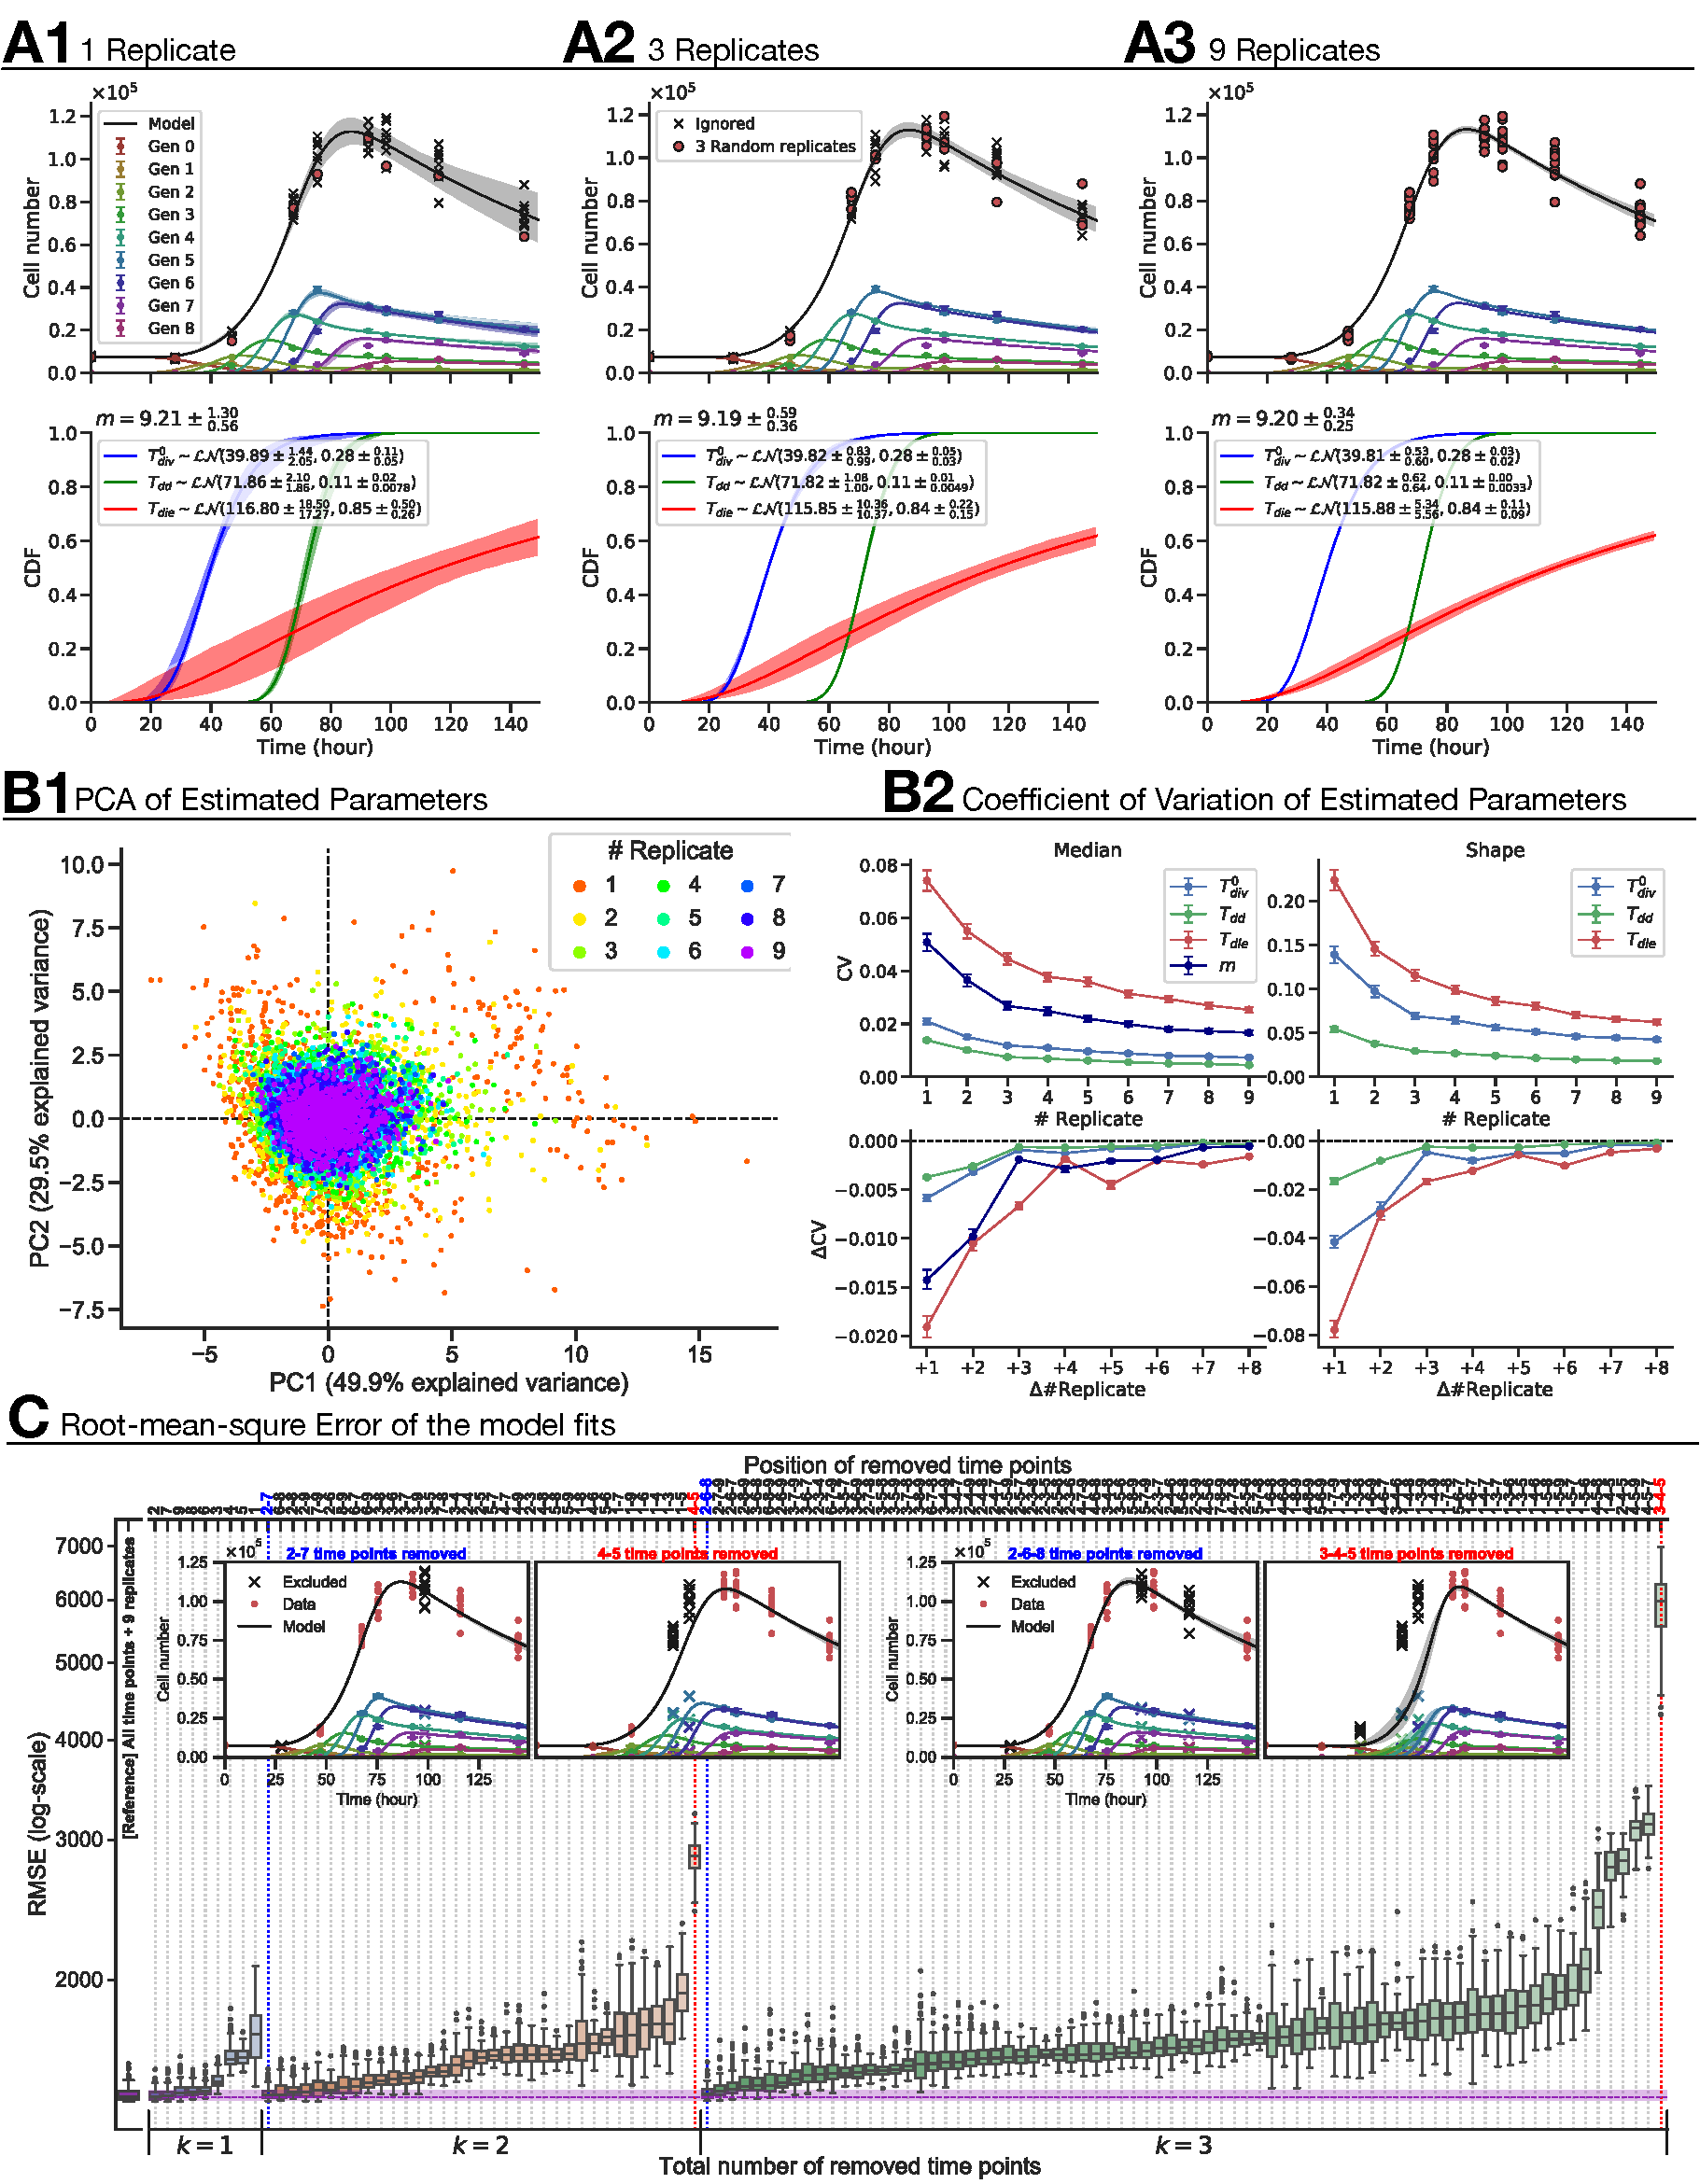
\includegraphics[scale=0.58]{figs/fig5.pdf}
    \caption{\textbf{The precision of parameter estimation and accuracy of the model fit with CpG-stimulated Bim$^{-/-}$ murine B cell data.} \textbf{(A1-3)} The best-fit model extrapolation (\textit{top}) and its corresponding estimated parameters (\textit{bottom}). For a given replicate number, $10^3$ artifical datsets were created by randomly sampling the original dataset with replacement per time point and fitted to calculate 95\% confidence bands. \textbf{(B1)} From the sets of estimated parameter vectors, marginal coefficients of variation (CV) was calculated with 95\% confidence interval from bootstrapping. \textbf{(B2)} Principle component analysis (PCA) of the estimated parameter vectors. \textbf{(C)} Root-mean-square error (RMSE) evaluated over all time points and replicates after fitting the model to artificially removed datasets. Examples of the best (\textit{blue}) and worst (\textit{red}) fits are shown.}
    \label{fig:Bcell_application}
\end{figure}
\clearpage

\nolinenumbers
\subsection{T cells: Additive nature of signal integration in time domain}
\begin{figure}[t]
    \centering
    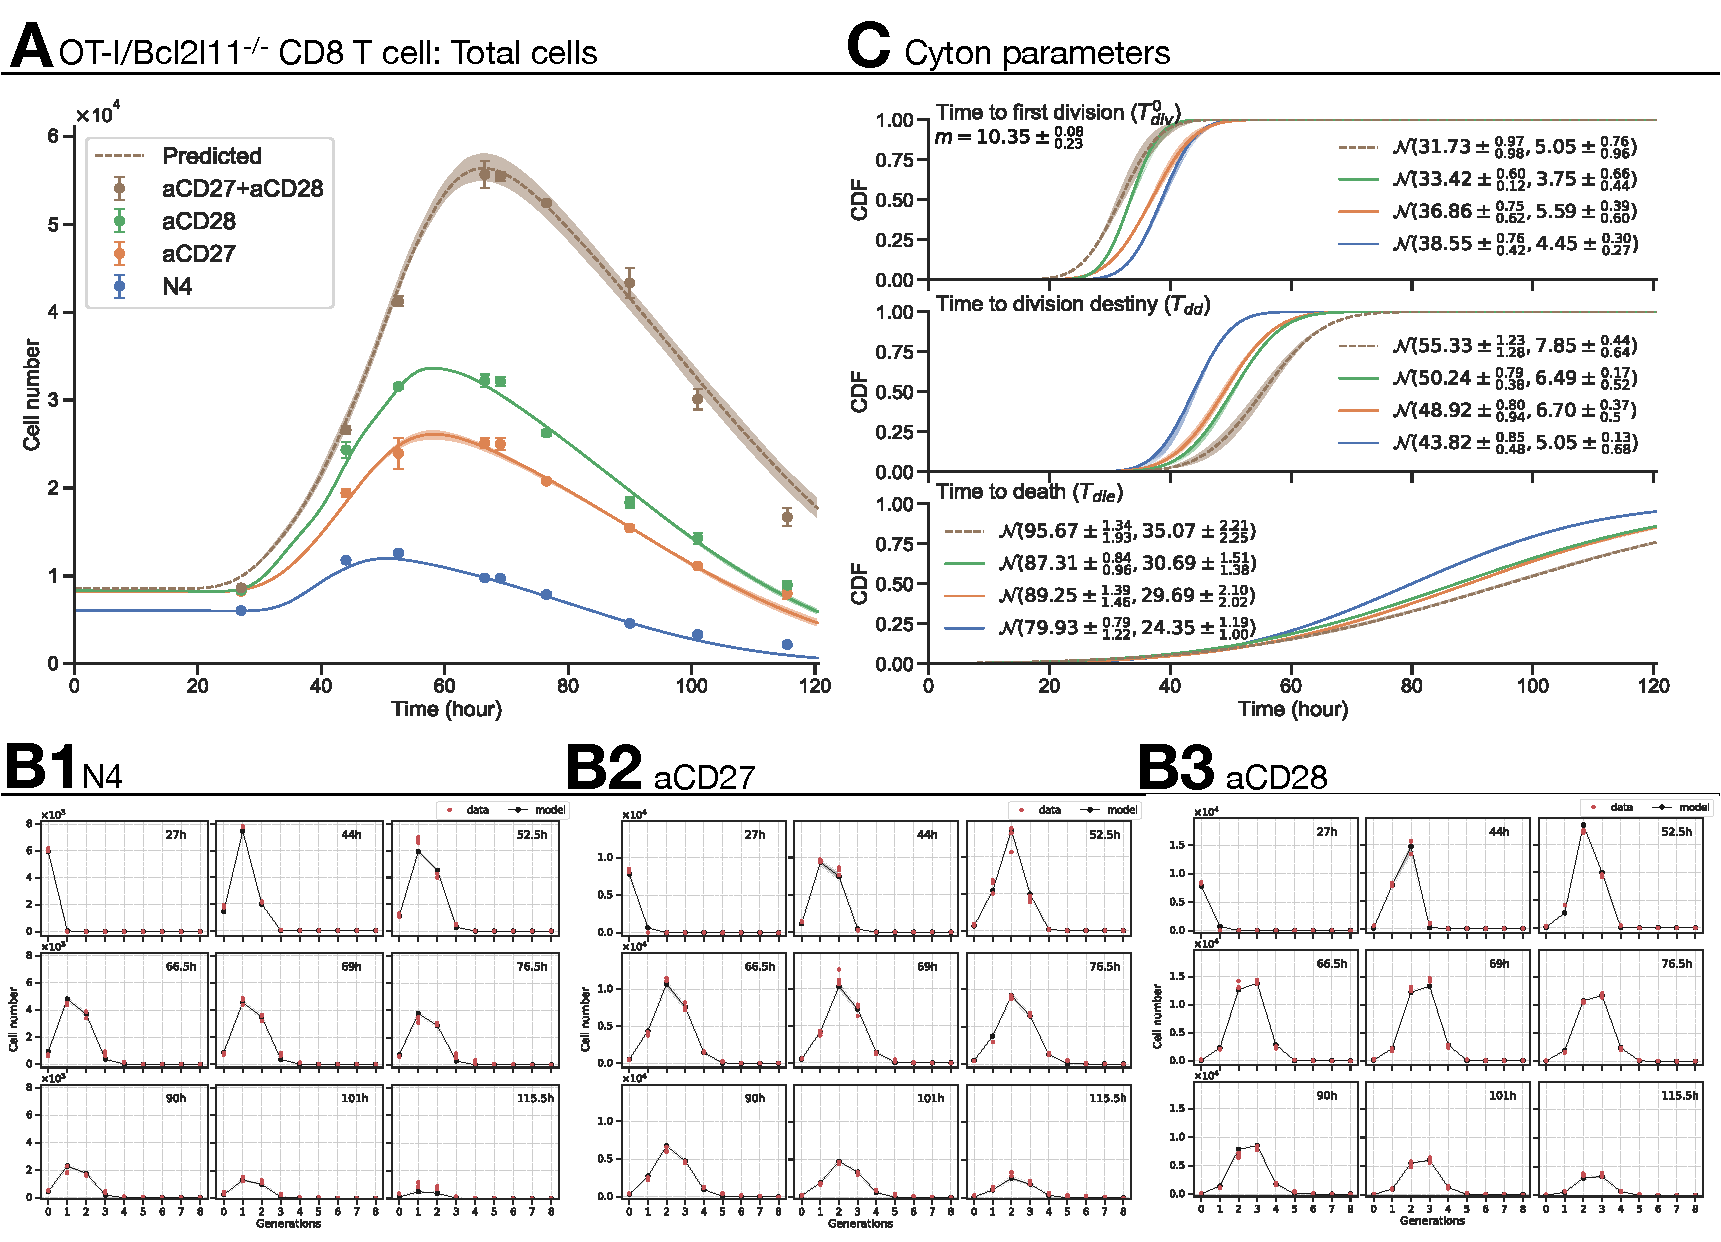
\includegraphics[scale=0.6]{figs/fig6.pdf}
    \caption{\textbf{Cyton2 fitting to FACS T cell data \parencite{Marchingo.2014}.} The cells were stimulated with N4 (\textit{blue}) as basis for all other conditions. \textbf{(A)} Harvested total cell numbers ($\bullet$: mean $\pm$ SEM) overlaid with the model extrapolation and 95\% confidence band from bootstrapping. \textbf{(B1-3)} Live cells per generation and the model extrapolation at harvested time points. \textbf{(C)} Estimated parameters of $m, T_{div}^0, T_{dd}, T_{die}$ and their 95\% confidence intervals. The fitted and predicted values of mean and standard deviation are labelled in the legend for normally distributed random variables.}
    \label{fig:application}
\end{figure}
% \linenumbers
To further illustrate the model, we used it to capture the mean population dynamics of an experiment presented in \cite{Marchingo.2014}. This data was obtained from \textit{in vitro} CTV-labeled OT-I/Bcl2l11$^{-/-}$ CD8 T cells stimulated with N4 and cultured with antibodies of CD27 (5$\mu$g mL$^{-1}$) and CD28 (2$\mu$g mL$^{-1}$) alone and their combination. To accurately capture the effects of the stimuli, 25$\mu$g mL$^{-1}$ of S4B6, which blocks endogenous IL-2 produced interim, was added to all cultures. CD8 T cells were harvested at 27h, 44h, 52.5h, 66.5h, 69h, 76.5h, 90h, 101h and 115.5h after the stimulation with three replicates at each time point. Refer to the original article for more detail on the experiment setup.

\cite{Marchingo.2014} showed that each contribution of stimuli was manifested as an increase in mean division number (MDN) from the basis signal (N4). It was concluded that the effect of combination of two or more signals (e.g. aCD27+aCD28) is a simple linear sum of changes in MDN with respect to the basis signal from each component. Here, we asked if the same rule can be applied in the time domain that is, for example, $T_{dd}^{\mathrm{aCD27+aCD28}} = T_{dd}^{\mathrm{N4}} + \Delta T_{dd}^{\mathrm{aCD27}} + \Delta T_{dd}^{\mathrm{aCD28}}$, where $\Delta$ denotes for the change in $T_{dd}$ with respect to N4. To do so, we used \textit{normal} distribution for all variables in the model as there is no closed-form for sum of independent but not necessarily identical two or more lognormal distributions. Thus, assuming normally distributed random variables, we formulated a simple algebraic sum of the timers by,
\begin{linenomath*}
    \begin{equation}
        \label{eq:combined_timers}
        T_{\mathrm{aCD27+aCD28}} \sim \mathcal{N}\left(\mu_{\mathrm{N4}} + \Delta \mu_{\mathrm{aCD27}} + \Delta \mu_{\mathrm{aCD28}}, \sqrt{\sigma_{\mathrm{N4}}^2 + \Delta \sigma^2_{\mathrm{aCD27}} + \Delta \sigma^2_{\mathrm{aCD28}}}\right),
    \end{equation}
\end{linenomath*}
where $\Delta \mu_x = \mu_x - \mu_{\mathrm{N4}}$ and $\Delta \sigma_x^2 = \sigma_x^2 - \sigma_{\mathrm{N4}}^2$.

In \cref{fig:application}A, we present total cell numbers and the best-fit model with 95\% confidence band around the estimate from the original data (see Methods). The model was simultaneously fitted to N4, aCD27 and aCD28 datasets with a shared subsequent division time (\cref{fig:application}B1-3). The estimated $m$ and cumulative distribution functions (CDF) of $T_{div}^0$, $T_{dd}$ and $T_{die}$ are shown in \cref{fig:application}C. In comparison to N4 alone, the addition of aCD27 and aCD28 extends both means of $T_{dd}$ ($\approx$15\%) and $T_{die}$ ($\approx$10\%). Also, we identified aCD28 reduces mean of $T_{div}^0$ (13.3\%) while aCD27 has minimal impact. Collectively, the compounding effect of these changes results in larger expansion of cell numbers by letting cells to enter the first division early and to reach destiny and death at later times. Given the estimates of parameters for N4, aCD27 and aCD28, we predicted the cell numbers for their combined effect by calculating the $T_{div}^0, T_{dd}$ and $T_{die}$ according to \cref{eq:combined_timers}. Strikingly, we successfully recreated the expansion kinetics of OT-I/Bcl2l11$^{-/-}$ CD8 T cells in the presence of both aCD27 and aCD28 (\cref{fig:application}A), supporting the signal integration as a linear sum in a time domain and the independence of the timers. Additionally, we recapitulated the results in \cite{Marchingo.2014} by simulating the family trees using ABM given the fitted and predicted parameter values (\cref{supp_fig:recapitulate_application}). 

\nolinenumbers
\section{Discussion}
% \linenumbers
To date with the exception of quorum sensing models \parencite{Kannan.2018, Weber.2013}, essentially all of the lymphocyte proliferation models employed assumption that newly born cell's fate is independent of its family's history, and, of the lifetimes exponentially distributed \parencite{Mazzocco.2017, Banks.2012, Hasenauer.2012, Lee.2009, Yates.2007, Ganusov.2005, Revy.2001, Nordon.1999, Smith.1973}, with a few notable exceptions (e.g. Cyton model, \cite{Yates.2017, Shokhirev.2015, Hyrien.2010, Zilman.2010, Wellard.2010}). These assumptions are adopted, not because they are consistent with experimental data from, for example, filming, FACS and multiplex, but for reasons of parsimony, model identifiability and computational ease of fitting. %Here, we introduce a new model, called Cyton2, where family correlation are included. This is done, however, in a way by which identifiability is improved while computational burden is not increased.
Here, we have formulated a variant of the original Cyton model that encapsulates feature of inheritance and correlation structure of cell fates. This was achieved by introducing new parameters called time to division destiny, which operates independent of the other cellular machinery, and global death time, which describes a single death time for all members in a family tree. Similar to the Cyton model, this variant offers a general tool for analysing lymphocyte proliferation and survival, particularly from the data obtained from CFSE/CTV-labeled division tracking assays. The formula for its computation turned out to be in a relatively simple form, despite the violation of a standard assumption (e.g. in the theory of branching process) that the progeny are stochastically independent entities. As a result, we believe that this simplicity improves the model identifiability while computational complexity is not increased. 

The analysis of the B and T cell filming data provided additional layer of consistency with the independence assumption of the cellular machineries, reassuring the very foundation of the Cyton model. We illustrated this by simulating large number of family trees under the independent operation of Cyton2 machineries. It was apparent that the censorship of the events rendered challenges in proving the assumption, however, we recapitulated the data to show its consistency, albeit not a definitive proof. Additionally, we identified the best parametric distribution class for essential variables of the Cyton2 model. Although the true governing distribution may not be possible to obtain, we inferred that lognormal distribution is the best descriptor of the timers, even for the time to division destiny. However, the normal distribution may be used to approximate the timers as well.

To capture the mean population dynamics, we have derived a formula that parameterised by a constant and three random variables, where three random variables represent times to first division, to division destiny and to death, and a constant is for subsequent division time equally applied to all generations after the first. We provided examples of the model utilisation for both B and T cells and illustrated that it equally well captured the dynamics, which has potential to offer as a general tool for other types of lymphocyte studies. Our main conclusions through studies of B and T cells are that firstly, the design of an experiment has an impact on the precision of parameter estimates and accuracy of the model. We recommend at least three replicates per experiment, which then can be further interrogated for confidence intervals via bootstrapping, and carefully select the harvested time points to ensure that the data contains at least one time point for each key events (e.g. expansion and/or contraction) in an experiment. Secondly, we further extended the work of \cite{Marchingo.2014} to show that the additive nature of T cell stimuli can also be expressed as a linear sum of normally distributed random variables that resides in time domain. This was verified by using Cyton2 model and ABM simulation, and we reached the same conclusion. One of limitations we wish to raise is that the support of a normal distribution can extend to negative infinity. This poses a challenge that it is mathematically possible to obtain negative mean values, and our study may had been a special case for more general rule. For this reason and together with evidence from the filming data, a lognormal distribution remains as an optimal choice for further investigation. To date, there is no closed-form expression to calculate sums of independent but not identical lognormal distributions. Moreover, there is no guarantee that the sum is a lognormal distribution. However, numerical approximations \parencite{Mehta.2007, Lo.2012} could be used as an initial point of attack.

One of generalisations of the model can be achieved by replacing the constant subsequent division time to a random variable. It is evident from the filming data that there exists some degrees of variation in division times for subsequent generations. However, our current proposed model fails to capture this behaviour. In this sense, more accurate description of lymphocyte proliferation remains as a challenge that may be investigated in future work.

% Precise manipulation and understanding of how each costimulation and cytokine signal integrate to generate T cell responses are important aspects in many of therapeutic applications such as immunotherapy for cancer treatment.

\nolinenumbers
\section{Methods}
% \linenumbers

\nolinenumbers
\subsection{Time-lapse Microscope}
\textcolor{red}{[Detailed experiment protocols for the filming data. I need help for this section... For B- and T-cell data, I have briefly explained the experiment setup in the main text and referred her original paper for more detail.]}
% \linenumbers

\nolinenumbers
\subsection{Data selection and tree collapse}
\begin{table}[h]
    \resizebox{\textwidth}{!}{%
    \begin{tabular}{@{}cccccc@{}}
    \toprule
    \multirow{2}{*}{\begin{tabular}[c]{@{}c@{}}Cell Type\end{tabular}} &
      \multicolumn{1}{c}{\multirow{2}{*}{Stim.}} &
      \multicolumn{4}{c}{Number of families for each variables} \\
     &
      \multicolumn{1}{c}{} &
      Time to fist division ($T_{div}^0$) &
      Subsequent division time ($M$) &
      Time to last division ($T_{ld}$) &
      Time to death ($T_{die}$) \\ \cmidrule(l){1-2} \cmidrule(l){3-3} \cmidrule(l){4-4} \cmidrule(l){5-5} \cmidrule(l){6-6}
    B &
      CpG &
      \begin{tabular}[c]{@{}c@{}}69 (63.9\%)\end{tabular} &
      \begin{tabular}[c]{@{}c@{}}56 (51.9\%)\end{tabular} &
      \begin{tabular}[c]{@{}c@{}}69 (63.9\%)\end{tabular} &
      \begin{tabular}[c]{@{}c@{}}69 (63.9\%)\end{tabular} \\ \midrule
    \multirow{3}{*}{\begin{tabular}[c]{@{}c@{}}CD8 T\\ (+IL2)\end{tabular}} &
      1U &
      \begin{tabular}[c]{@{}c@{}}28 (25.7\%)\end{tabular} &
      \begin{tabular}[c]{@{}c@{}}4 (3.7\%)\end{tabular} &
      \begin{tabular}[c]{@{}c@{}}28 (25.7\%)\end{tabular} &
      \begin{tabular}[c]{@{}c@{}}28 (25.7\%)\end{tabular} \\
     &
      3U &
      \begin{tabular}[c]{@{}c@{}}34 (37.8\%)\end{tabular} &
      \begin{tabular}[c]{@{}c@{}}13 (14.4\%)\end{tabular} &
      \begin{tabular}[c]{@{}c@{}}34 (37.8\%)\end{tabular} &
      \begin{tabular}[c]{@{}c@{}}34 (37.8\%)\end{tabular} \\
     &
      10U &
      \begin{tabular}[c]{@{}c@{}}50 (30.7\%)\end{tabular} &
      \begin{tabular}[c]{@{}c@{}}16 (9.8\%)\end{tabular} &
      \begin{tabular}[c]{@{}c@{}}50 (30.7\%)\end{tabular} &
      \begin{tabular}[c]{@{}c@{}}60 (30.7\%)\end{tabular} \\
      \bottomrule
    \end{tabular}%
    }
    \caption{\textbf{Number of clones retained after the filtering.}}
    \label{tab:data}
\end{table}
% \linenumbers
\noindent
For each family tree $c \in \mathbbm{N}_{\geq 0}$, the times to divide $\{T_{div}^x\}_c$, to die $\{T_{die}^x\}_c$ and to loss $\{T_{loss}^x\}_c$ of all cells were recorded using time-lapse microscope. $T_{loss}$ is defined as the time at which the cell becomes indistinguishable to the nearby cells, or survives until the end of given experiment time frame, thus, were lost from the experiment. In order to keep track of the cells' relation, a unique label was given to each cell by $x$. For example, we denote a founder cell $x = \cell{0}$, and its two daughter cells $x = \cell{1}$ and ${x = \cell{2}}$ so that, in general, $x = \cell{x_1, x_2, \dots, x_j}$ with $x_j \in \{1, 2\}$ would represent $x_j^\mathrm{th}$ daughter cell of $\dots$ of $x_2^{\mathrm{th}}$ daughter cell (see, \cite[Ch.6]{Harris.1963}). Let $\mathcal{X}_c$ be the collection of all $x$ for a family $c$. Given a unique identifier of the cell, its generation $k$ is extracted by $g(x) \coloneqq k$ with $g(\cell{0}) = 0$. With this construct, we define the raw measurement of times as a set $\mathcal{T}_c = \{t(x) \in \{T_{div}^x, T_{die}^x, T_{loss}^x\} : x \in \mathcal{X}_c\}$.

For analyses in \cref{sec:independence_of_timers} and \cref{sec:distribution_class}, we filtered for families that had at least divided once and satisfy $\max(\mathcal{T}_c) = T_{die}^x$ condition. In essence, we eliminated incomplete family trees that contain unusually long-surviving cells, but allowed unrecovered cells to be in place as long as the last observed event is death in a given family. Indeed there is increasing chance of observing more lost cells as family grows larger. However, it was previously shown that the regularity of a family is a result of correlated cell divisions as a biological feature inherited within the family even when considering the unrecovered samples \parencite{Marchingo.2016}. Therefore, it is highly likely that the lost cells due to indistinguishable circumstance might had undergone similar fates with its sibling, thereby maximising the number of data points while reducing any potential selection bias, whereas it is difficult to weigh how including the long-surviving cells might affect all the other analyses.

Given the heritability feature, we summarise a family tree by collapsing it to a single representative line (\cref{fig:model}C). By collapsing we mean substitute average time to divide (and to die) of the cells in a given generation $k$, that is
\begin{linenomath*}
    \begin{equation*}
        T_{div}^k \coloneqq \frac{\sum_{\{x:g(x)=k\}}T_{div}^x}{|\{x:g(x)=k\}|}, \quad T_{die}^k \coloneqq \frac{\sum_{\{x:g(x)=k\}}T_{die}^x}{|\{x:g(x)=k\}|}.
    \end{equation*}
\end{linenomath*}
We also enumerated all dead cells within a family and calculated mean time to last division ($T_{ld}$) as a proxy to the division destiny time. In summary, we represent a single family by $\mathbf{T}(c) = (T_{div}^0, \cdots, T_{div}^k, T_{die}^0, \dots, T_{die}^k)$ so long as we observed division or death events in each generation $k$.  \cref{tab:data} shows the number of retained families used in all analyses presented in this paper given $\mathbf{T}(c)$ after applying the filtering rule.

\nolinenumbers
\subsection{Agent-Based Model}
% \linenumbers
We developed an agent-based model (ABM) to simulate cells in a single family with the correlated structured proposed for the Cyton2 model. Each realisation of the simulation represents one clonal family. Upon initialisation, the founder cell is assigned time to first division, global destiny and global death times, which were drawn randomly from three independent lognormal distribution. The time taken to the subsequent division after the first is also randomly drawn from a lognormal distribution, but it remains constant and equally applied for all subsequent generations. If the founder cell reaches time to first division, it creates two daughter cells, which inherit global destiny and death times. 
%If the cell reaches destiny but has progressed more than one third of total division time within its generation, it is allowed to divide one more time \parencite{Dowling.2014}, otherwise we immediately classify it as a destiny cell and prevent from further division. 
If the cell reaches destiny we immediately classify if as a destiny cell and prevent from further division. When the cells reach death time they are removed from the simulation. The model was implemented in \verb+Python+ (version 3.8.6).


\nolinenumbers
\subsection{Statistical Analysis: Bayesian Framework}
% \linenumbers
The correlations of every pair of time to first division ($T_{div}^0$), average subsequent division time ($M$), time to last division ($T_{ld}$) and time to death ($T_{die}$) were estimated using Bayesian inference. For a given pair of variables and its observed data, say $d_i \in \mathcal{D} = \{(x_i, y_i) : i=1,2,\dots,n\}$ where $n$ is the number of observations, we used bivariate normal distribution to capture the correlation ($\rho$). This entails $x_i \sim N(\mu_x, \sigma_x)$ and $y_i \sim N(\mu_y, \sigma_y)$. With uninformative priors on the hyper parameters $\mu_x, \mu_y \sim U(0, 1000)$, $\sigma_x, \sigma_y \sim U(0, 1000)$ and $\rho \sim U(-1, 1)$, we define the bivariate normal distribution,
\begin{linenomath*}
    \begin{equation*}
        d_i \sim N(\boldsymbol{\mu}, \mathbf{\Sigma}),
    \end{equation*}
\end{linenomath*}
where $\boldsymbol{\mu} = (\mu_x, \mu_y)$ is a vector of means for $x_i$ and $y_i$, and $\mathbf{\Sigma} = \begin{bmatrix*} \sigma_x^2 & \rho \sigma_x \sigma_y \\ \rho \sigma_x \sigma_y & \sigma_y^2 \end{bmatrix*}$ is a covariance matrix. We used an extension of Hamiltonian MCMC algorithm, No-U-Turn Sampler \parencite{Hoffman.2011}, implemented in \verb+PyMC3+ \parencite{Salvatier.2016} to infer the posterior distributions of $\rho, \mu_x, \sigma_x, \mu_y, \sigma_y$. Given these distributions, we calculated 95\% credible interval for $\rho$, and 90\%, 95\% and 99\% density regions of ($x, y$). In addition to this, we can formulate bayesian hypothesis testing, where the null hypothesis is $H_0$: $\rho=0$ and alternative hypothesis is $H_1$: $\rho \neq 0$ (which translates to $H_1$: $\rho \sim U(-1, 1)$) \parencite{Jeffreys.1961}. This is formally stated as a ratio of likelihoods of hypotheses given the data,
\begin{linenomath*}
    \begin{equation*}
        \frac{P(H_0 | \mathcal{D})}{P(H_1 | \mathcal{D})} = \frac{P(H_0)}{P(H_1)} \times \frac{P(\mathcal{D} | H_0)}{P(\mathcal{D} | H_1)}.
    \end{equation*}
\end{linenomath*}
In order to grade if the data is more probable under $H_0$ or $H_1$, the Bayes factor BF$_{01} = P(\mathcal{D} | H_0)/P(\mathcal{D} | H_1)$ was used given priors of $P(H_0)$ and $P(H_1)$. When $H_1$: $\rho \sim U(-1,1)$, it can be computed by evaluating the following integral \parencite{Jeffreys.1961, Wagenmakers.2016}:
\begin{linenomath*}
    \begin{equation*}
        \mathrm{BF}_{01} = 1/\mathrm{BF}{_{10}}, \text{ where } \mathrm{BF}_{10} = \frac{1}{2}\int_{-1}^{1} \frac{(1 - \rho^2)^{\frac{n-1}{2}}}{(1 - \rho r)^{n-\frac{3}{2}}} d\rho,
    \end{equation*}
\end{linenomath*}
where $r$ denotes for the sample correlation defined as $r = \sum_{i=1}^n (x_i - \bar{x}) (y_i - \bar{y})/\sqrt{\sum_{i=1}^n (x_i - \bar{x})^2 \sum_{i=1}^n (y_i - \bar{y})^2}$. \cref{tab:bayes_factor_interpretation} shows the discrete categories of evidential strength proposed in \cite{Jeffreys.1961} for the interpretation of the Bayes factor. The analysis was applied in \cref{sec:independence_of_timers} and \cref{sec:censorship}.
\begin{table}[h]
    % \resizebox{\textwidth}{!}{%
    \centering
    \begin{tabular}{@{}cl@{}}
        \toprule
        Bayes Factor: BF$_{01}$ (BF$_{10}$) & Interpretation                         \\ \cmidrule(l){1-1} \cmidrule(l){2-2}
        \textgreater{}100                   & Extreme evidence for $H_0$ ($H_1$)     \\
        30 - 100                            & Very strong evidence for $H_0$ ($H_1$) \\
        10 - 30                             & Strong evidence for $H_0$ ($H_1$)      \\
        1 - 3                               & Anecdotal evidence for $H_0$ ($H_1$)   \\
        1                                   & No evidence      \\                 
        \bottomrule    
    \end{tabular}
    % }
    \caption{\textbf{Bayes factor interpretation.}}
    \label{tab:bayes_factor_interpretation}
\end{table}

In \cref{sec:distribution_class}, the candidates of parametric distribution class were assessed for $T_{div}^0, M, T_{ld}, T_{die}$ variables under the Bayesian framework in a similar manner to estimating the correlation coefficient. \cref{tab:candidate_distribution} shows the list of candidate distributions and the uninformative priors prescribed for respective parameters. 
\begin{table}[h]
    % \resizebox{\textwidth}{!}{%
    \centering
    \begin{tabular}{@{}ccl@{}}
        \toprule
        Candidates & Priors & Target Distribution \\ \cmidrule(l){1-1} \cmidrule(l){2-2} \cmidrule(l){3-3}
        A & $\alpha_G, \beta_G \sim U(0,200)$ & $T_{div}^0, M, T_{ld}, T_{die} \sim \mathrm{Gamma}(\alpha_G, \beta_G)$ \\
        B & $m, s \sim U(0,200)$ & $T_{div}^0, M, T_{ld}, T_{die} \sim \mathrm{LN}(m, s)$ \\
        C & $\mu, \sigma \sim U(0,200)$ & $T_{div}^0, M, T_{ld}, T_{die} \sim \mathrm{N}(\mu, \sigma)$ \\
        D & $\alpha_W, \beta_W \sim \mathrm{HalfNormal}(0, 200)$ & $T_{div}^0, M, T_{ld}, T_{die} \sim \mathrm{Weibull}(\alpha_W, \beta_W)$ \\
        \bottomrule    
    \end{tabular}
    % }
    \caption{\textbf{List of candidate parametric distribution classes.}}
    \label{tab:candidate_distribution}
\end{table}
Given posterior distributions of the parameters, we adopted WAIC \parencite{Watanabe.2010} score to quantitatively assess the candidates, which is estimated as follows:
\begin{linenomath*}
    \begin{equation*}
        \mathrm{WAIC}(z, \Theta) = -2 \left(\sum_{i=1}^n \log\left[\frac{1}{S} \sum_{s=1}^S P(z_i|\Theta_s)\right] - \sum_{i=1}^n \mathrm{Var}_{s=1}^S \log(P(z_i|\Theta_s)) \right),
    \end{equation*}
\end{linenomath*}
where $z$ is the data with $n$ independent number of observations, $\Theta$ is the posterior distribution,  $\Theta_s$ is the $s$-th set of sampled parameter values in the posterior distribution with $S$ number of samples and $\mathrm{Var}_{s=1}^S a_s = \frac{1}{S-1} \sum_{s=1}^S (a_s - \bar{a})^2$ denotes for the sample variance  \parencite{McElreath.2020, Vehtari.2017}. The first and the second terms in $(\cdot)$ are known as the \textit{log-pointwise-predictive-density} (lppd) and the penalty term, respectively. For direct comparison of the candidates, we computed the standard error by calculating the variance over the individual observations instead of their summation under the assumption of normality of WAIC.
\begin{linenomath*}
    \begin{equation}
        \mathrm{se}(\mathrm{WAIC}) =\sqrt{n \times \mathrm{Var}_{i=1}^n \left( -2\log\left[\frac{1}{S} \sum_{s=1}^S P(z_i|\Theta_s)\right] + 2\mathrm{Var}_{s=1}^S \log(P(z_i|\Theta_s)) \right)}.
    \end{equation}
\end{linenomath*}
Let us denote $\mathrm{WAIC}_i$ to be the term in $\sqrt{(\cdot)}$ such that $\mathrm{WAIC} = \sum_{i=1}^n \mathrm{WAIC}_i$, then the standard error of the difference of WAIC between, for instance, candidate A and B can be calculated,
\begin{linenomath*}
    \begin{equation*}
        \mathrm{se}(\mathrm{WAIC}^A - \mathrm{WAIC}^B) =\sqrt{n \times \mathrm{Var}_{i=1}^n \left(\mathrm{WAIC}_i^A - \mathrm{WAIC}_i^B \right)}.
    \end{equation*}
\end{linenomath*}

\nolinenumbers
\subsection{Fitting Cyton Model}
% \linenumbers
Division structured population datasets obtained from FACS were fitted to the Cyton2 model (\cref{eq:final_expected_cell_number}). There are total of 7 parameters to be estimated for each dataset, thus if we have $N$ number of conditions, we have a maximum of $7N$ free parameters to be fitted. For all conditions, we always used cell numbers at the beginning of the stimulus (typically at $t=0$) as a fixed initial cell number.

For each set of cell numbers $\{n_{g,r}(t_i)\}$ from the data, where $i \in \{0, 1, \dots, I\}$, $g \in \{0, 1, \dots, G\}$ and $r \in \{0,1,\dots,R\}$ are time, generation and replicate indices, respectively, we obtained point estimates of the parameters. 
% To achieve this, we used least-squares method with two numerical optimisation algorithms to reduce chances of falling in local minima: Levenberg-Marquardt \parencite{Marquardt.1963} and Differential Evolution \parencite{Storn.1997} implemented in \verb+Python+ library \verb+LMFIT+ (version 1.0.1) \parencite{Newville.2014}. We ran two algorithms simultaneously and picked the best one according to the cost function
To achieve this, we used least-squares method with Levenberg-Marquardt \parencite{Marquardt.1963} optimisation algorithm implemented in \verb+Python+ library \verb+LMFIT+ (version 1.0.1) \parencite{Newville.2014}. We defined our cost function, 
\begin{linenomath*}
    \begin{equation*}
        C(\boldsymbol{\theta}) = \sum_{i=0}^I \sum_{g=0}^G \sum_{r=0}^{R} \left( n_{g,r}(t_i) - y_g(t_i; \boldsymbol{\theta}) \right)^2,
    \end{equation*}
\end{linenomath*}
such that we found an approximate minimum,
\begin{linenomath*}
    \begin{equation*}
        \{\boldsymbol{\theta}^*\} \in \operatorname*{arg\,min}_{\boldsymbol{\theta}} C(\boldsymbol{\theta}).
    \end{equation*}
\end{linenomath*}
As each algorithm requires a starting parameter value, we prescribed 100 sets of initial values drawn uniformly at random from the appropriate parameter ranges, and recorded residual sum-of-squares for each set to pick the best fitted parameters at the end. After identifying the best fit, we performed bootstrap method \parencite{Efron.1979} with an artificial dataset that was resampled with replacement (per time point) from the original measured data. We repeated this process 100 times, resulted in 100 additional estimates for each parameter. This allowed us to calculate 95\% confidence intervals on the best fitted parameter values. Additionally, we also obtained confidence bands for extrapolated cell numbers by calculating 95\% percentile range at each of discretised time point from the model.

\nolinenumbers
\section*{AUTHOR CONTRIBUTIONS}
% \linenumbers

\nolinenumbers
\section*{FUNDING}
% \linenumbers
This project has received funding from the European Union's Horizon 2020 research and innovation programme under the Marie Skłodowska-Curie grant agreement No 764698. This publication has emanated from research supported in part by a research grant from Science Foundation Ireland (SFI) under Grant Number 16/RI/3399.

\nolinenumbers
\section*{ACKNOWLEDGEMENTS}
% \linenumbers

\nolinenumbers


\nolinenumbers
\singlespacing
\newrefcontext[sorting=ydnt]
\printbibliography

\clearpage
\setcounter{figure}{0}
\setcounter{table}{0}
\setcounter{page}{1}
\renewcommand{\thepage}{S\arabic{page}}
\renewcommand{\thesection}{S\arabic{section}}
\renewcommand{\thetable}{S\arabic{table}}
\renewcommand{\thefigure}{S\arabic{figure}}
\section*{Supplementary Materials}
\label{sec:supplementary}

\begin{figure}[H]
    \centering
    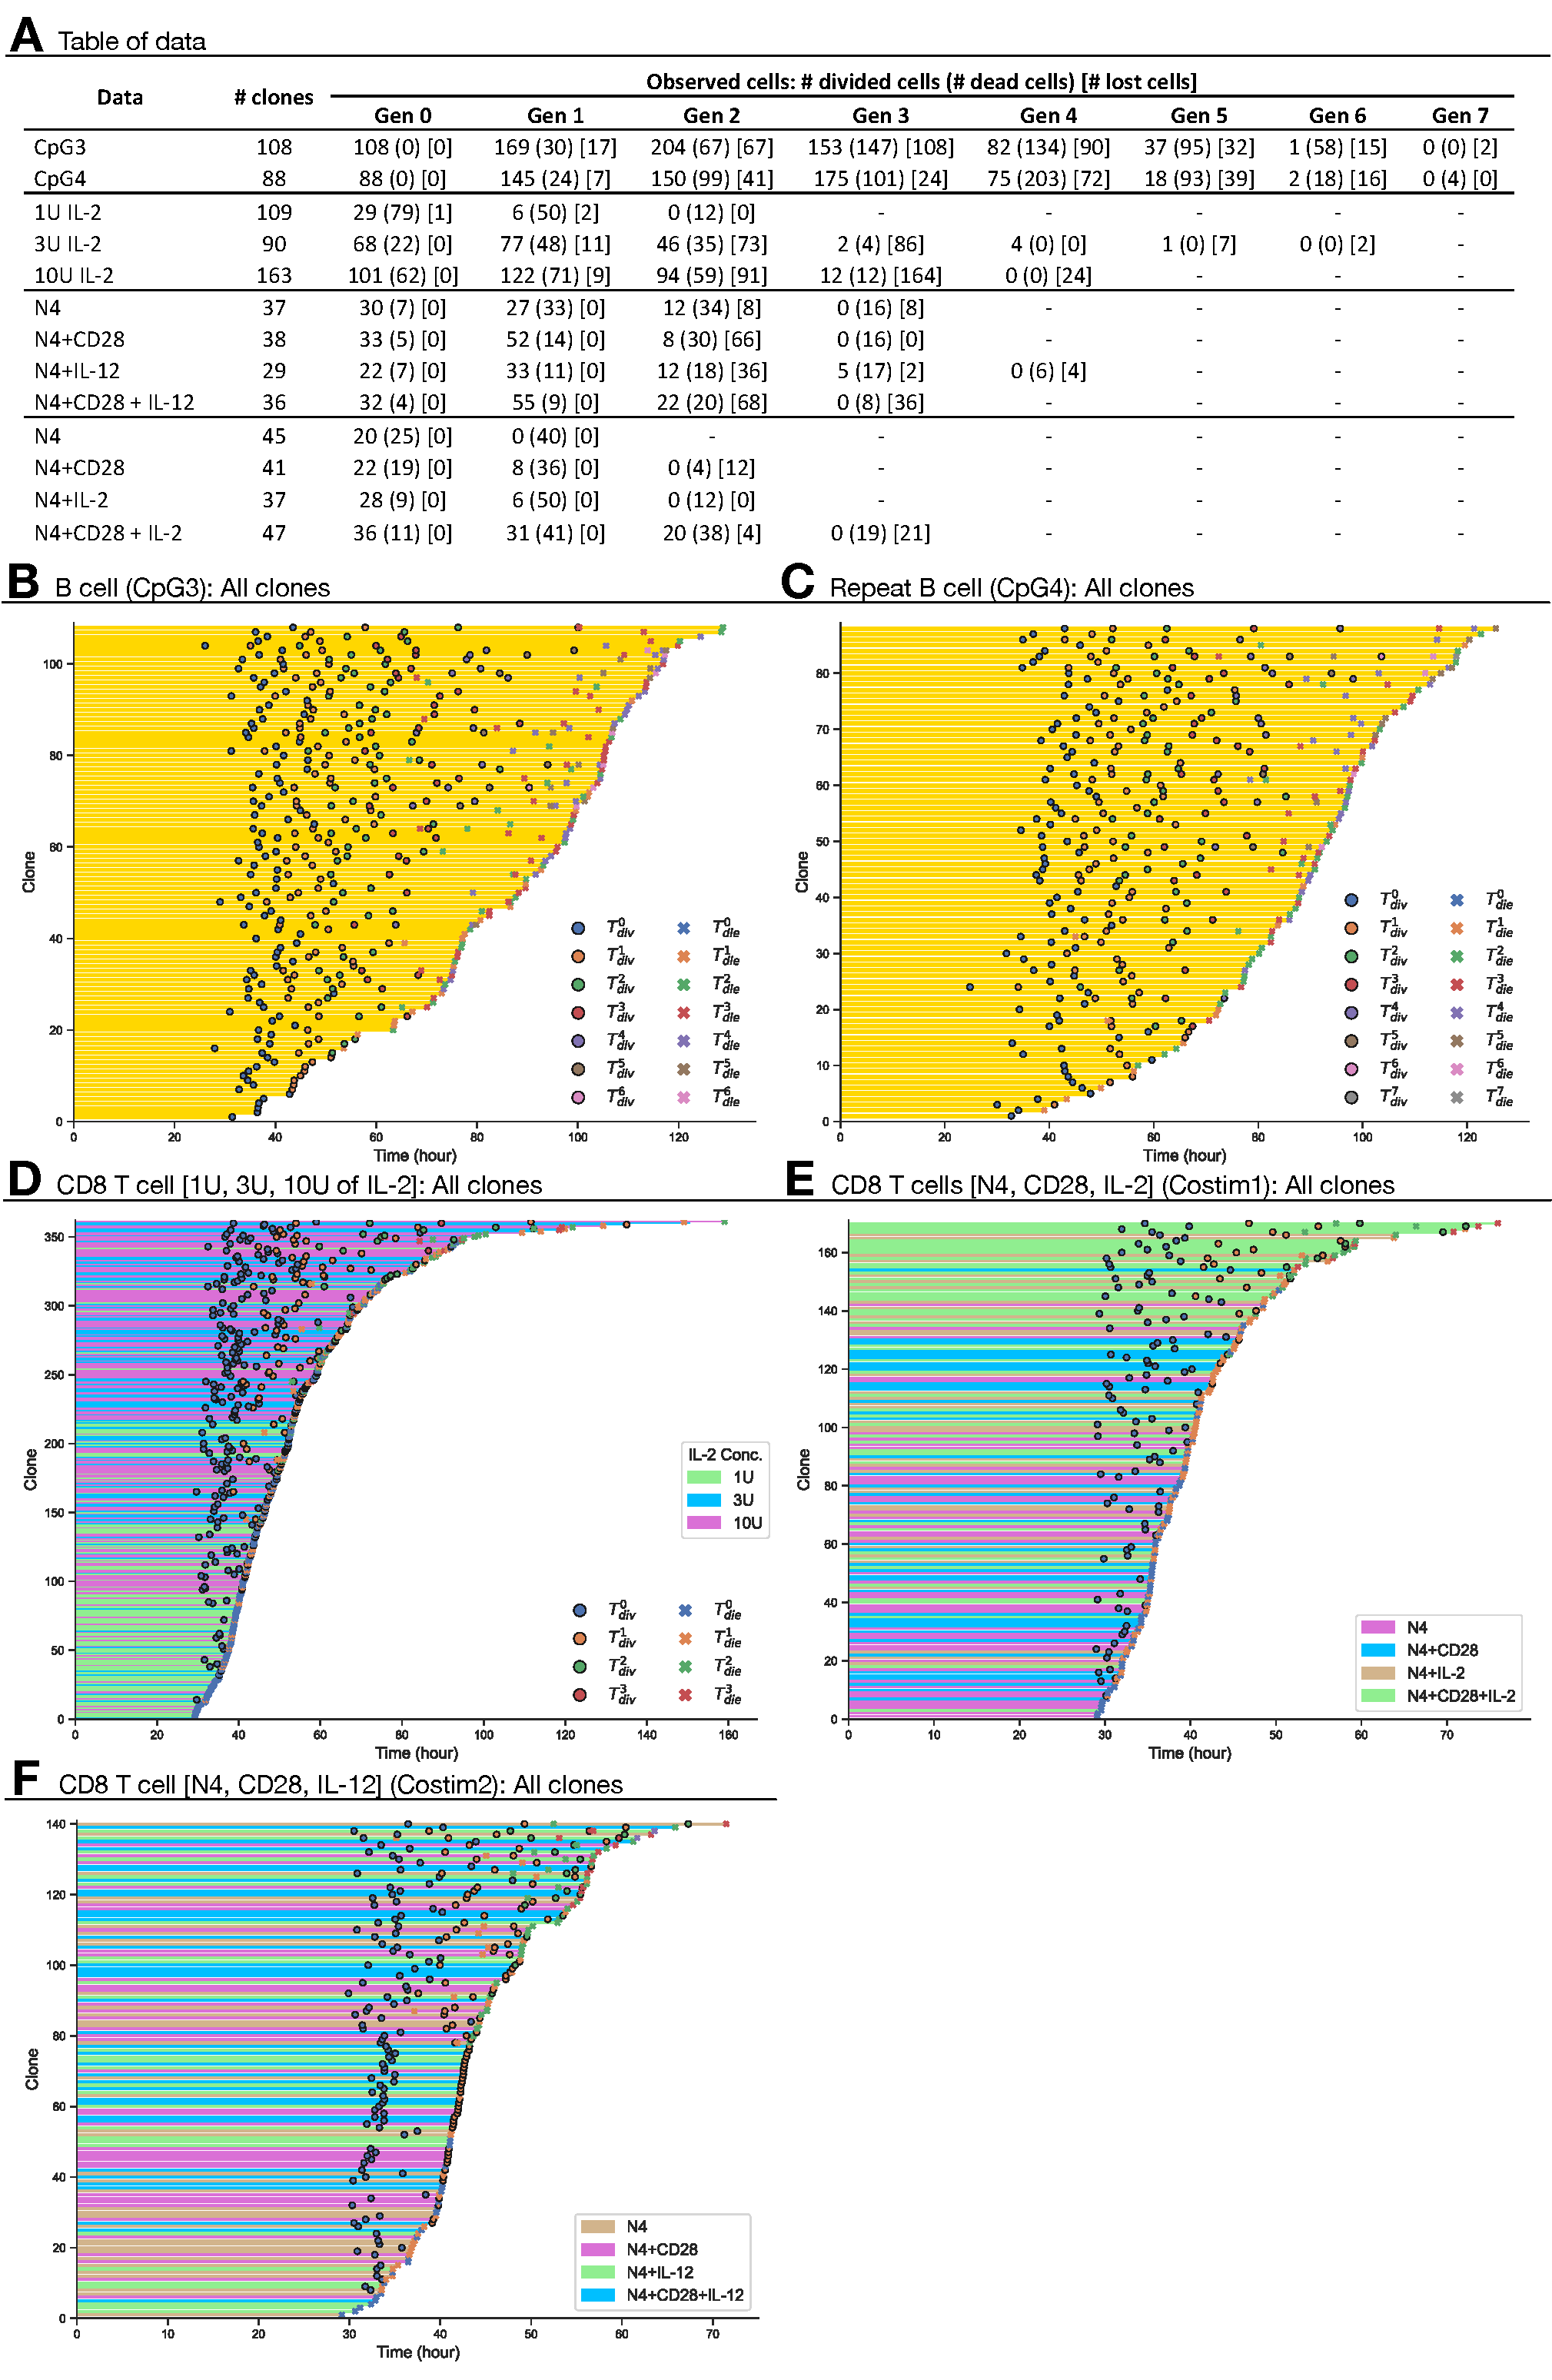
\includegraphics[scale=0.46]{figs/supp_fig1.pdf}
    \caption{\textbf{Raw filming data.} \textbf{(A)} Number of founder cells and raw numbers of observed divided, dead and lost cells at each generation are tabulated. \textbf{(B-F)} Clonally collapsed trees for all families before the filtering. The average division ($\bullet$) and death ($\times$) times are marked, where the colors represent generation that the event was observed. The lost times are not shown.}
    \label{supp_fig:raw_data}
\end{figure}

\clearpage
\begin{figure}[H]
    \centering
    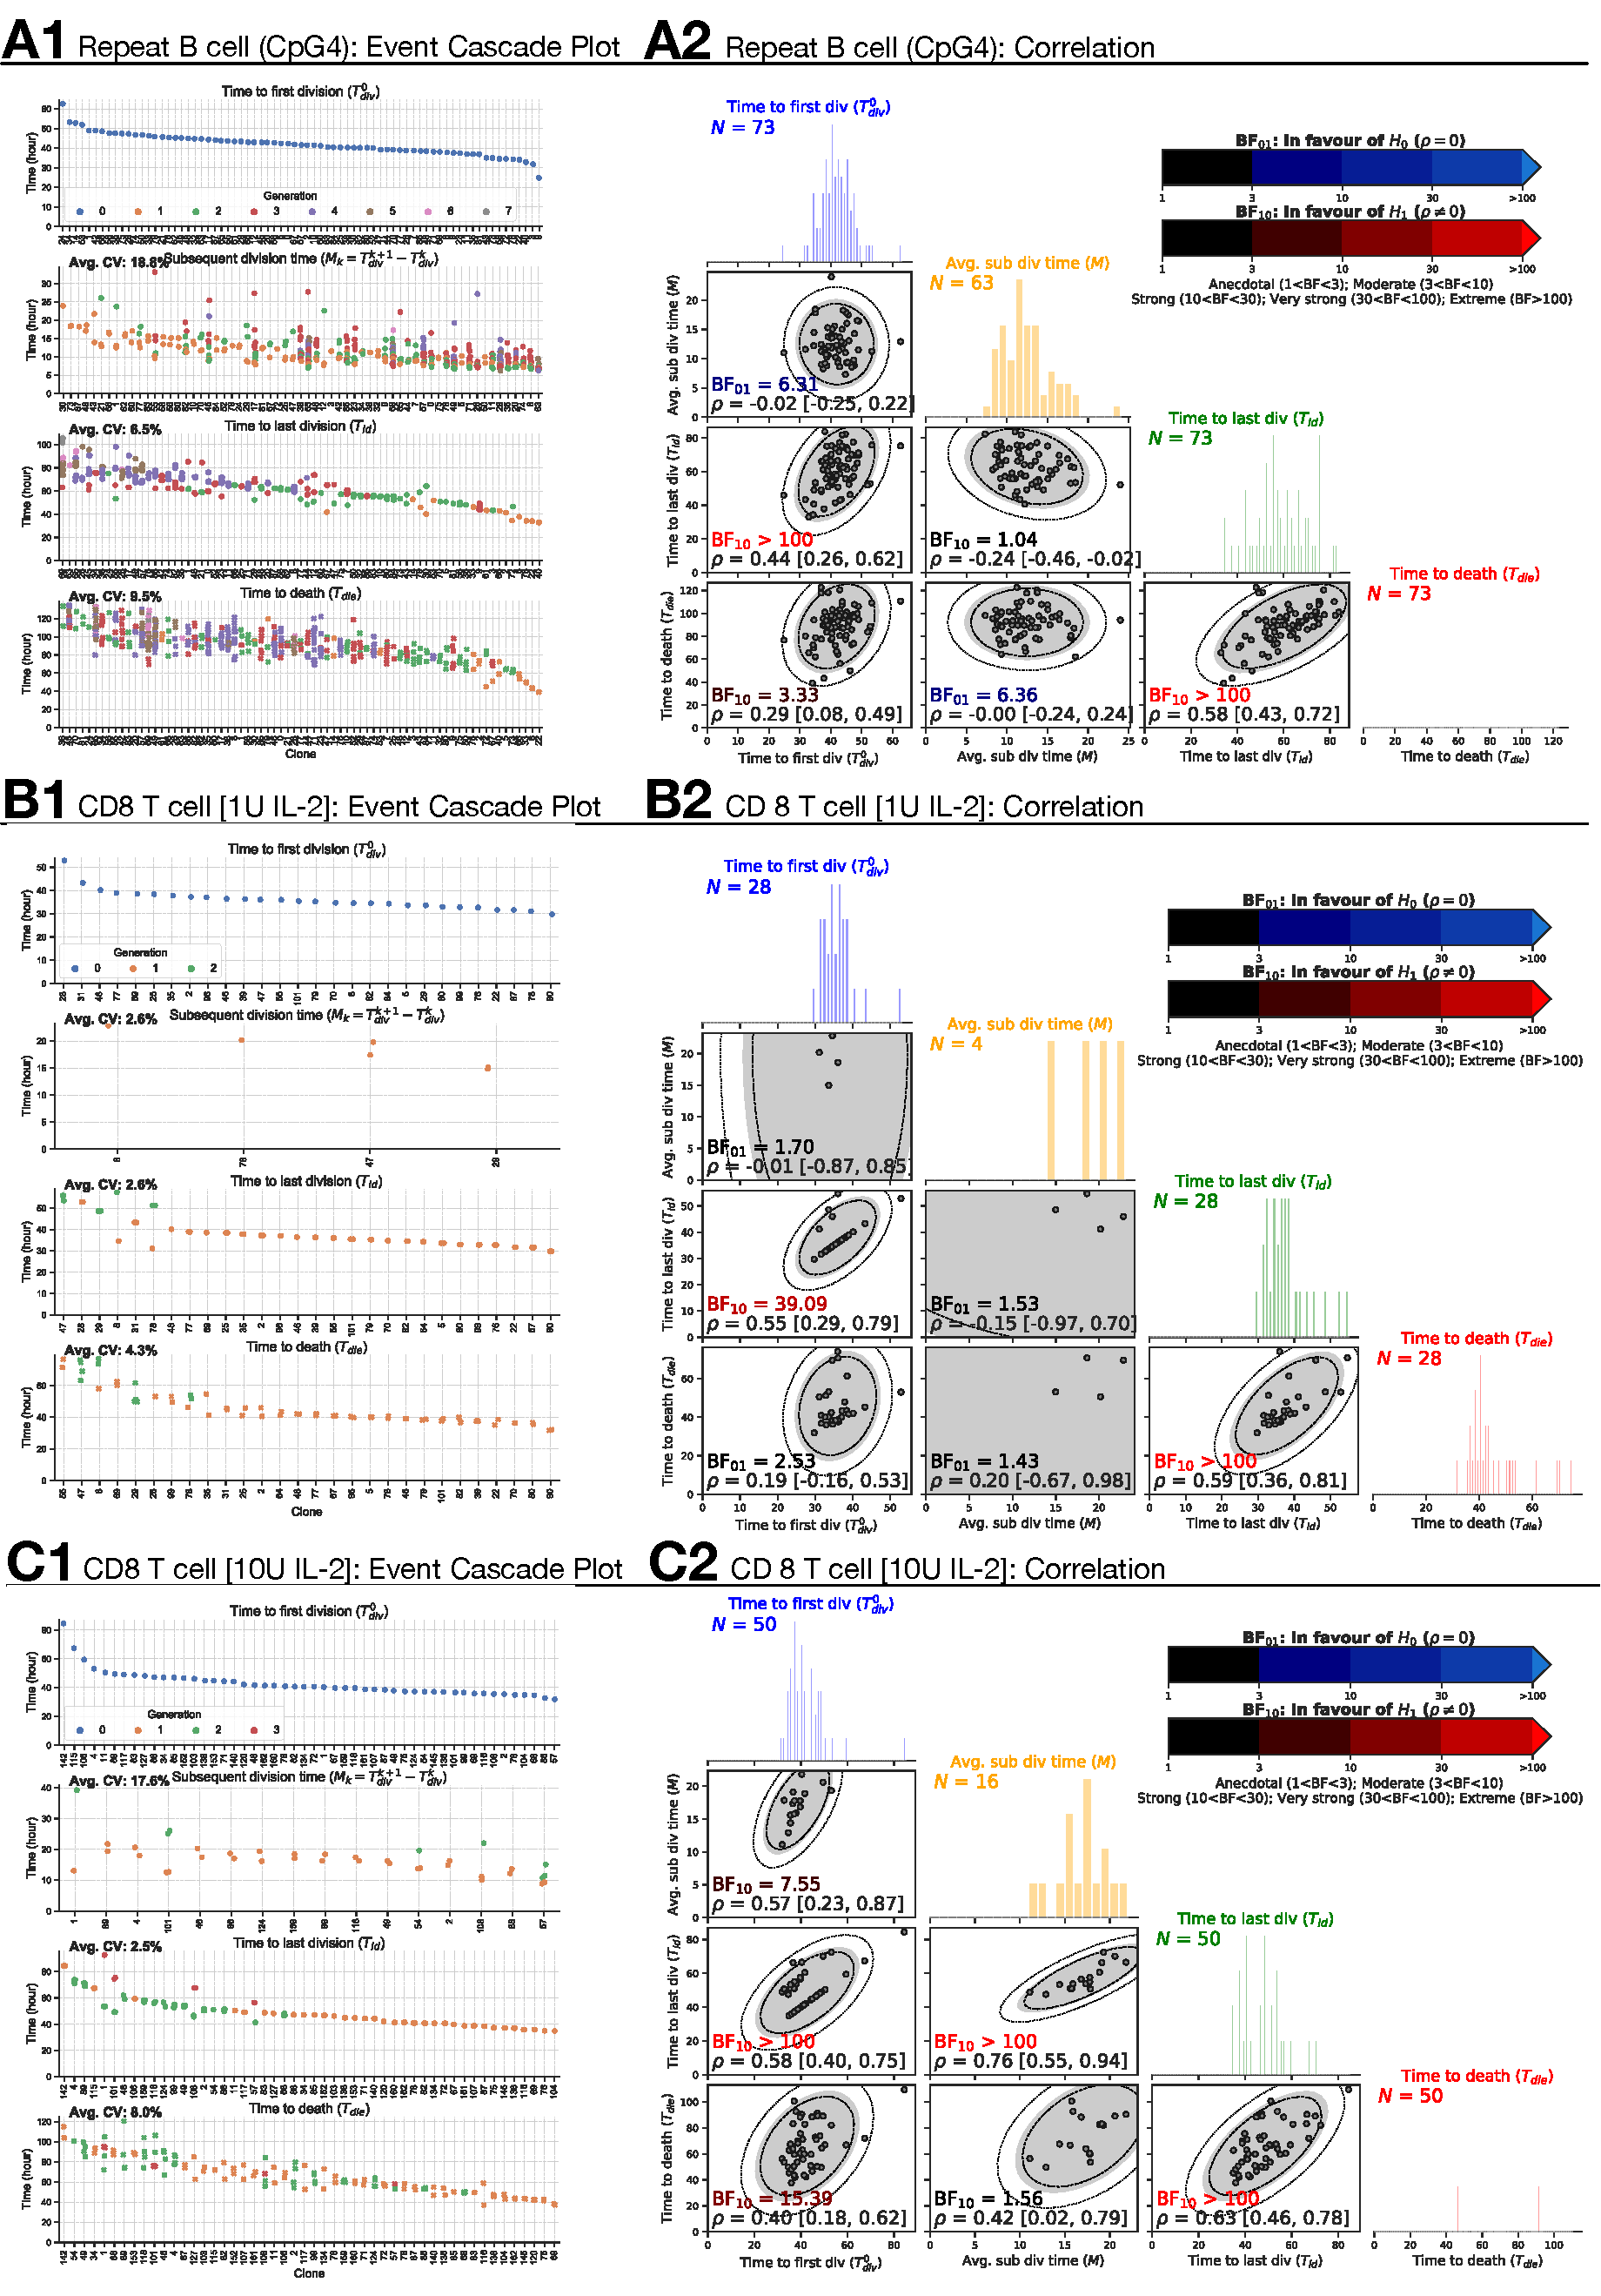
\includegraphics[scale=0.55]{figs/supp_fig2.pdf}
    \caption{\textbf{Extracting times to fates and the correlation analysis} \textbf{(A1-2)} Repeat of CpG-stimulated B cell (CpG4). \textbf{(B1-2)} CD8 T cells in the presence of 1U of IL-2. \textbf{(C1-2)} CD8 T cells in the presence of 10U of IL-2.}
    \label{supp_fig:repeats}
\end{figure}

\clearpage
\begin{figure}[H]
    \centering
    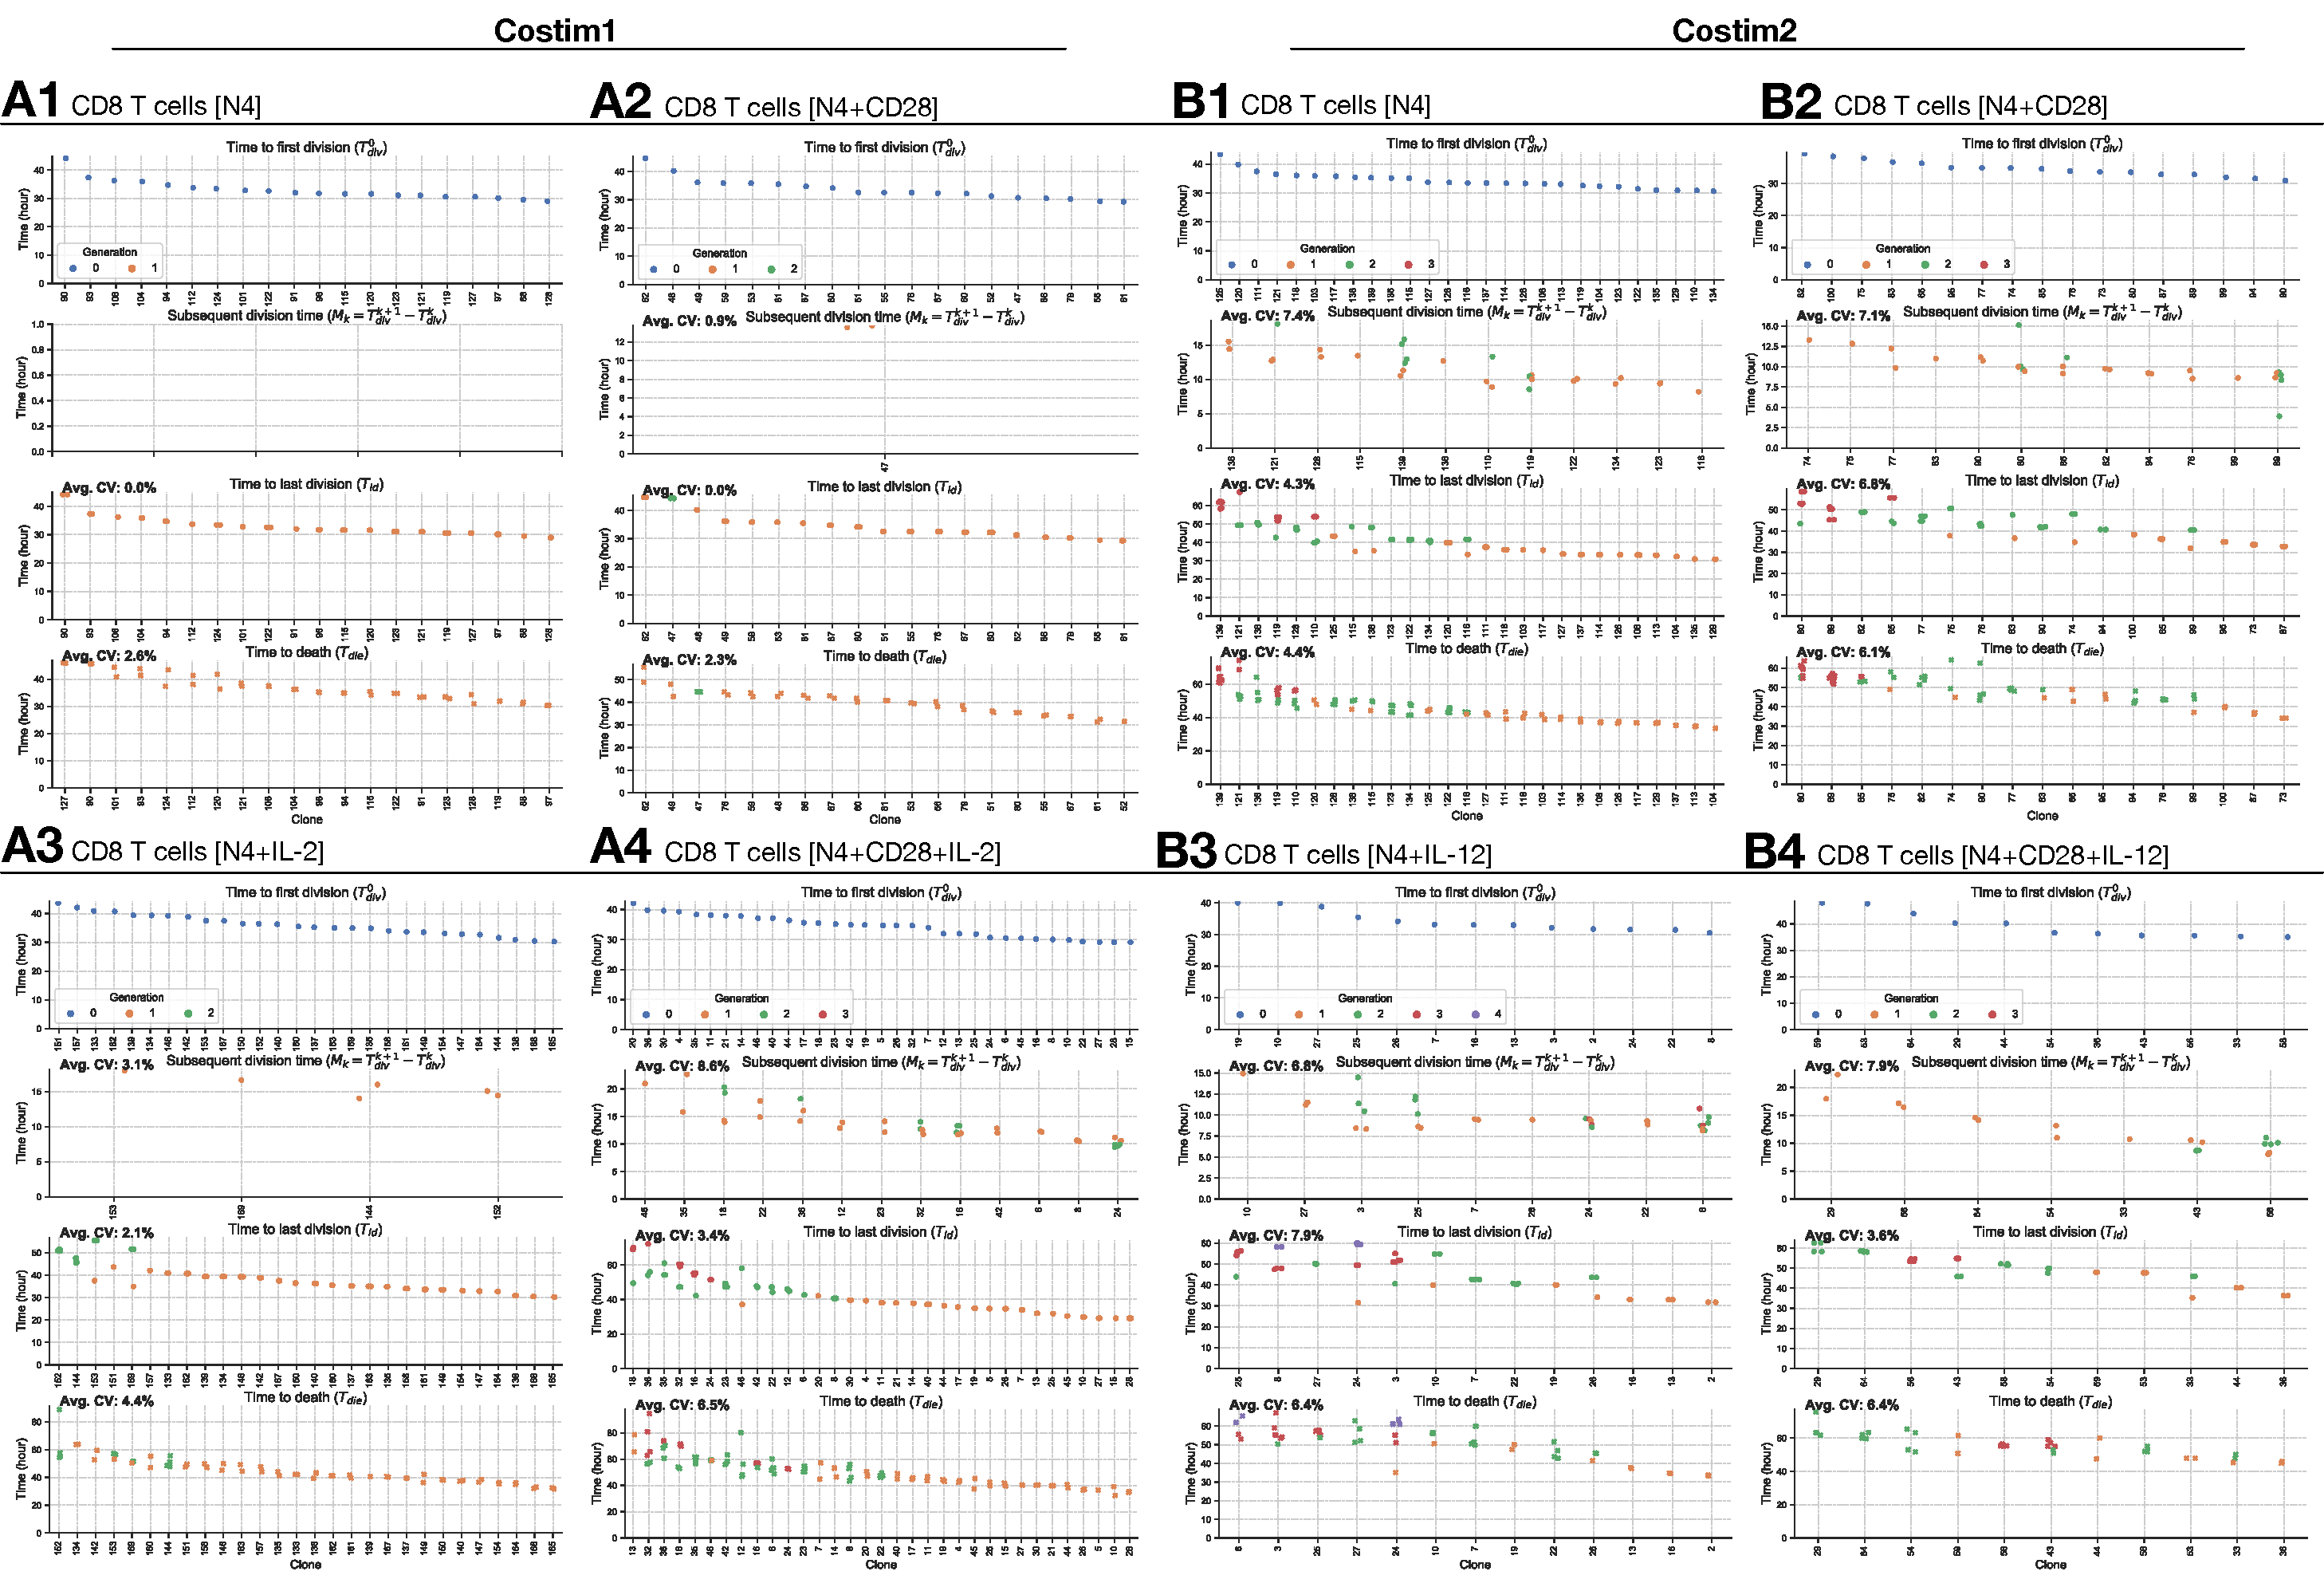
\includegraphics[scale=0.37]{figs/supp_fig3.pdf}
    \caption{\textbf{Extracting times to fates.} \textbf{(A1-4)} Experiment Costim1 consists of N4, N4+CD28, N4+IL-2 and N4+CD28+IL-2. \textbf{(B1-4)} Experiment Costim2 constists of N4, N4+CD28, N4+IL-12 and N4+CD28+IL-12.}
    \label{supp_fig:costims}
\end{figure}

\begingroup
\renewcommand{\arraystretch}{1.2}
\begin{table}[H]
    \resizebox{\textwidth}{!}{%
    \begin{tabular}{@{}clcccccc@{}}
    \toprule
    \multirow{2}{*}{\begin{tabular}[c]{@{}c@{}}Cell\\ Type\end{tabular}} &
      \multicolumn{1}{c}{\multirow{2}{*}{Stim.}} &
      \multicolumn{6}{c}{Bayes Factor (01/10) \& Correlation Coefficient ($\rho$ [CI])} \\
     &
      \multicolumn{1}{c}{} &
      ($T_{div}^0, M$) &
      ($T_{div}^0, T_{ld}$) &
      ($T_{div}^0, T_{die}$) &
      ($M, T_{ld}$) &
      ($M, T_{die}$) &
      ($T_{ld}, T_{die}$) \\ \cmidrule(l){1-2} \cmidrule(l){3-3} \cmidrule(l){4-4} \cmidrule(l){5-5} \cmidrule(l){6-6} \cmidrule(l){7-7} \cmidrule(l){8-8} 
    \multirow{4}{*}{\begin{tabular}[c]{@{}c@{}}CD8 T\\ (Costim1)\end{tabular}} &
      N4 &
      \begin{tabular}[c]{@{}c@{}}\textcolor{bf01_1}{NA}\end{tabular} &
      \begin{tabular}[c]{@{}c@{}}\textcolor{bf10_5}{\textgreater{}100 (10)}\\ 1.00 {[}1.00, 1.00{]}\end{tabular} &
      \begin{tabular}[c]{@{}c@{}}\textcolor{bf10_2}{8.31 (10)}\\ 0.53 {[}0.22, 0.82{]}\end{tabular} &
      \begin{tabular}[c]{@{}c@{}}\textcolor{bf01_1}{NA}\end{tabular} &
      \begin{tabular}[c]{@{}c@{}}\textcolor{bf01_1}{NA}\end{tabular} &
      \begin{tabular}[c]{@{}c@{}}\textcolor{bf10_2}{8.31 (10)}\\ 0.53 {[}0.22, 0.82{]}\end{tabular} \\
     &
      N4+CD28 &
      \begin{tabular}[c]{@{}c@{}}\textcolor{bf10_1}{NA}\end{tabular} &
      \begin{tabular}[c]{@{}c@{}}\textcolor{bf10_4}{85.63 (10)}\\ 0.67 {[}0.42, 0.89{]}\end{tabular} &
      \begin{tabular}[c]{@{}c@{}}\textcolor{bf10_3}{18.83 (10)}\\ 0.59 {[}0.30, 0.86{]}\end{tabular} &
      \begin{tabular}[c]{@{}c@{}}\textcolor{bf10_1}{NA}\end{tabular} &
      \begin{tabular}[c]{@{}c@{}}\textcolor{bf10_1}{NA}\end{tabular} &
      \begin{tabular}[c]{@{}c@{}}\textcolor{bf10_4}{60.52 (10)}\\ 0.66 {[}0.39, 0.89{]}\end{tabular} \\
     &
      N4+IL-2 &
      \begin{tabular}[c]{@{}c@{}}\textcolor{bf01_1}{1.30 (01)}\\ 0.24 {[}-0.63, 0.99{]}\end{tabular} &
      \begin{tabular}[c]{@{}c@{}}\textcolor{bf10_2}{29.98 (10)}\\ 0.54 {[}0.28, 0.78{]}\end{tabular} &
      \begin{tabular}[c]{@{}c@{}}\textcolor{bf10_1}{2.09 (10)}\\ 0.38 {[}0.07, 0.68{]}\end{tabular} &
      \begin{tabular}[c]{@{}c@{}}\textcolor{bf01_1}{1.31 (01)}\\ -0.24 {[}-0.99, 0.64{]}\end{tabular} &
      \begin{tabular}[c]{@{}c@{}}\textcolor{bf01_1}{1.58 (01)}\\ -0.12 {[}-0.96, 0.73{]}\end{tabular} &
      \begin{tabular}[c]{@{}c@{}}\textcolor{bf10_5}{\textgreater{}100 (10)}\\ 0.69 {[}0.49, 0.86{]}\end{tabular} \\
     &
      N4+CD28+IL-2 &
      \begin{tabular}[c]{@{}c@{}}\textcolor{bf10_2}{4.17 (10)}\\ 0.55 {[}0.17, 0.88{]}\end{tabular} &
      \begin{tabular}[c]{@{}c@{}}\textcolor{bf10_1}{1.03 (10)}\\ 0.30 {[}-0.01, 0.59{]}\end{tabular} &
      \begin{tabular}[c]{@{}c@{}}\textcolor{bf01_2}{3.28 (01)}\\ 0.14 {[}-0.18, 0.46{]}\end{tabular} &
      \begin{tabular}[c]{@{}c@{}}\textcolor{bf01_1}{1.26 (01)}\\ 0.33 {[}-0.14, 0.77{]}\end{tabular} &
      \begin{tabular}[c]{@{}c@{}}\textcolor{bf01_1}{1.77 (01)}\\ 0.26 {[}-0.22, 0.73{]}\end{tabular} &
      \begin{tabular}[c]{@{}c@{}}\textcolor{bf10_5}{\textgreater{}100 (10)}\\ 0.71 {[}0.54, 0.86{]}\end{tabular} \\ \midrule
      \multirow{4}{*}{\begin{tabular}[c]{@{}c@{}}CD8 T\\ (Costim2)\end{tabular}} &
      N4 &
      \begin{tabular}[c]{@{}c@{}}\textcolor{bf10_2}{15.12 (10)}\\ 0.68 {[}0.36, 0.94{]}\end{tabular} &
      \begin{tabular}[c]{@{}c@{}}\textcolor{bf01_1}{2.04 (01)}\\ 0.22 {[}-0.13, 0.56{]}\end{tabular} &
      \begin{tabular}[c]{@{}c@{}}\textcolor{bf01_1}{2.31 (01)}\\ 0.20 {[}-0.15, 0.54{]}\end{tabular} &
      \begin{tabular}[c]{@{}c@{}}\textcolor{bf10_1}{2.69 (10)} \\ 0.52 {[}0.10, 0.89{]}\end{tabular} &
      \begin{tabular}[c]{@{}c@{}}\textcolor{bf10_2}{3.53 (10)} \\ 0.55 {[}0.15, 0.90{]}\end{tabular} &
      \begin{tabular}[c]{@{}c@{}}\textcolor{bf10_5}{\textgreater{}100 (10)}\\ 0.95 {[}0.91, 0.98{]}\end{tabular} \\
     &
      N4+CD28 &
      \begin{tabular}[c]{@{}c@{}}\textcolor{bf01_1}{1.34 (01)} \\ 0.33 {[}-0.17, 0.79{]}\end{tabular} &
      \begin{tabular}[c]{@{}c@{}}\textcolor{bf01_1}{2.84 (01)}\\ 0.13 {[}-0.31, 0.57{]}\end{tabular} &
      \begin{tabular}[c]{@{}c@{}}\textcolor{bf01_1}{2.75 (01)}\\ 0.14 {[}-0.30, 0.58{]}\end{tabular} &
      \begin{tabular}[c]{@{}c@{}}\textcolor{bf01_1}{2.82 (01)} \\ -0.02 {[}-0.55, 0.52{]}\end{tabular} &
      \begin{tabular}[c]{@{}c@{}}\textcolor{bf01_1}{1.48 (01)} \\ 0.30 {[}-0.20, 0.77{]}\end{tabular} &
      \begin{tabular}[c]{@{}c@{}}\textcolor{bf10_5}{\textgreater{}100 (10)}\\ 0.83 {[}0.67, 0.96{]}\end{tabular} \\
     &
      N4+IL-12 &
      \begin{tabular}[c]{@{}c@{}}\textcolor{bf10_3}{14.97 (10)}\\ 0.74 {[}0.40, 0.98{]}\end{tabular} &
      \begin{tabular}[c]{@{}c@{}}\textcolor{bf01_1}{2.58 (01)}\\ 0.13 {[}-0.38, 0.63{]}\end{tabular} &
      \begin{tabular}[c]{@{}c@{}}\textcolor{bf01_1}{2.39 (01)}\\ 0.17 {[}-0.33, 0.66{]}\end{tabular} &
      \begin{tabular}[c]{@{}c@{}}\textcolor{bf01_1}{2.21 (01)}\\ 0.14 {[}-0.46, 0.74{]}\end{tabular} &
      \begin{tabular}[c]{@{}c@{}}\textcolor{bf01_1}{2.24 (01)}\\ 0.13 {[}-0.47, 0.73{]}\end{tabular} &
      \begin{tabular}[c]{@{}c@{}}\textcolor{bf10_5}{\textgreater{}100 (10)}\\ 0.95 {[}0.88, 0.99{]}\end{tabular} \\
     &
      N4+CD28+IL-12 &
      \begin{tabular}[c]{@{}c@{}}\textcolor{bf01_1}{1.33 (01)}\\ 0.32 {[}-0.33, 0.91{]}\end{tabular} &
      \begin{tabular}[c]{@{}c@{}}\textcolor{bf01_1}{2.47 (01)}\\ 0.12 {[}-0.43, 0.66{]}\end{tabular} &
      \begin{tabular}[c]{@{}c@{}}\textcolor{bf01_1}{2.48 (01)}\\ 0.12 {[}-0.44, 0.66{]}\end{tabular} &
      \begin{tabular}[c]{@{}c@{}}\textcolor{bf01_1}{1.00 (01)}\\ 0.40 {[}-0.22, 0.94{]}\end{tabular} &
      \begin{tabular}[c]{@{}c@{}}\textcolor{bf10_1}{1.16 (10)}\\ 0.44 {[}-0.18, 0.95{]}\end{tabular} &
      \begin{tabular}[c]{@{}c@{}}\textcolor{bf10_3}{29.19 (10)}\\ 0.74 {[}0.45, 0.96{]}\end{tabular} \\
      \bottomrule
    \end{tabular}%
    }
    \caption{\textbf{Test correlation of every pair of times to fates.} The Bayes factor and correlation coefficient calculated from a bivariate normal distribution with its 95\% credible interval is shown for CD8 T cell in combination of N4, CD28, IL2 (Costim1) and of N4, CD28, IL12 (Costim2). Minimum of two observations per variable pair was required for the calculation.}
    \label{tab:costim_independence}
\end{table}
\endgroup

\clearpage
\begin{figure}[h]
    \centering
    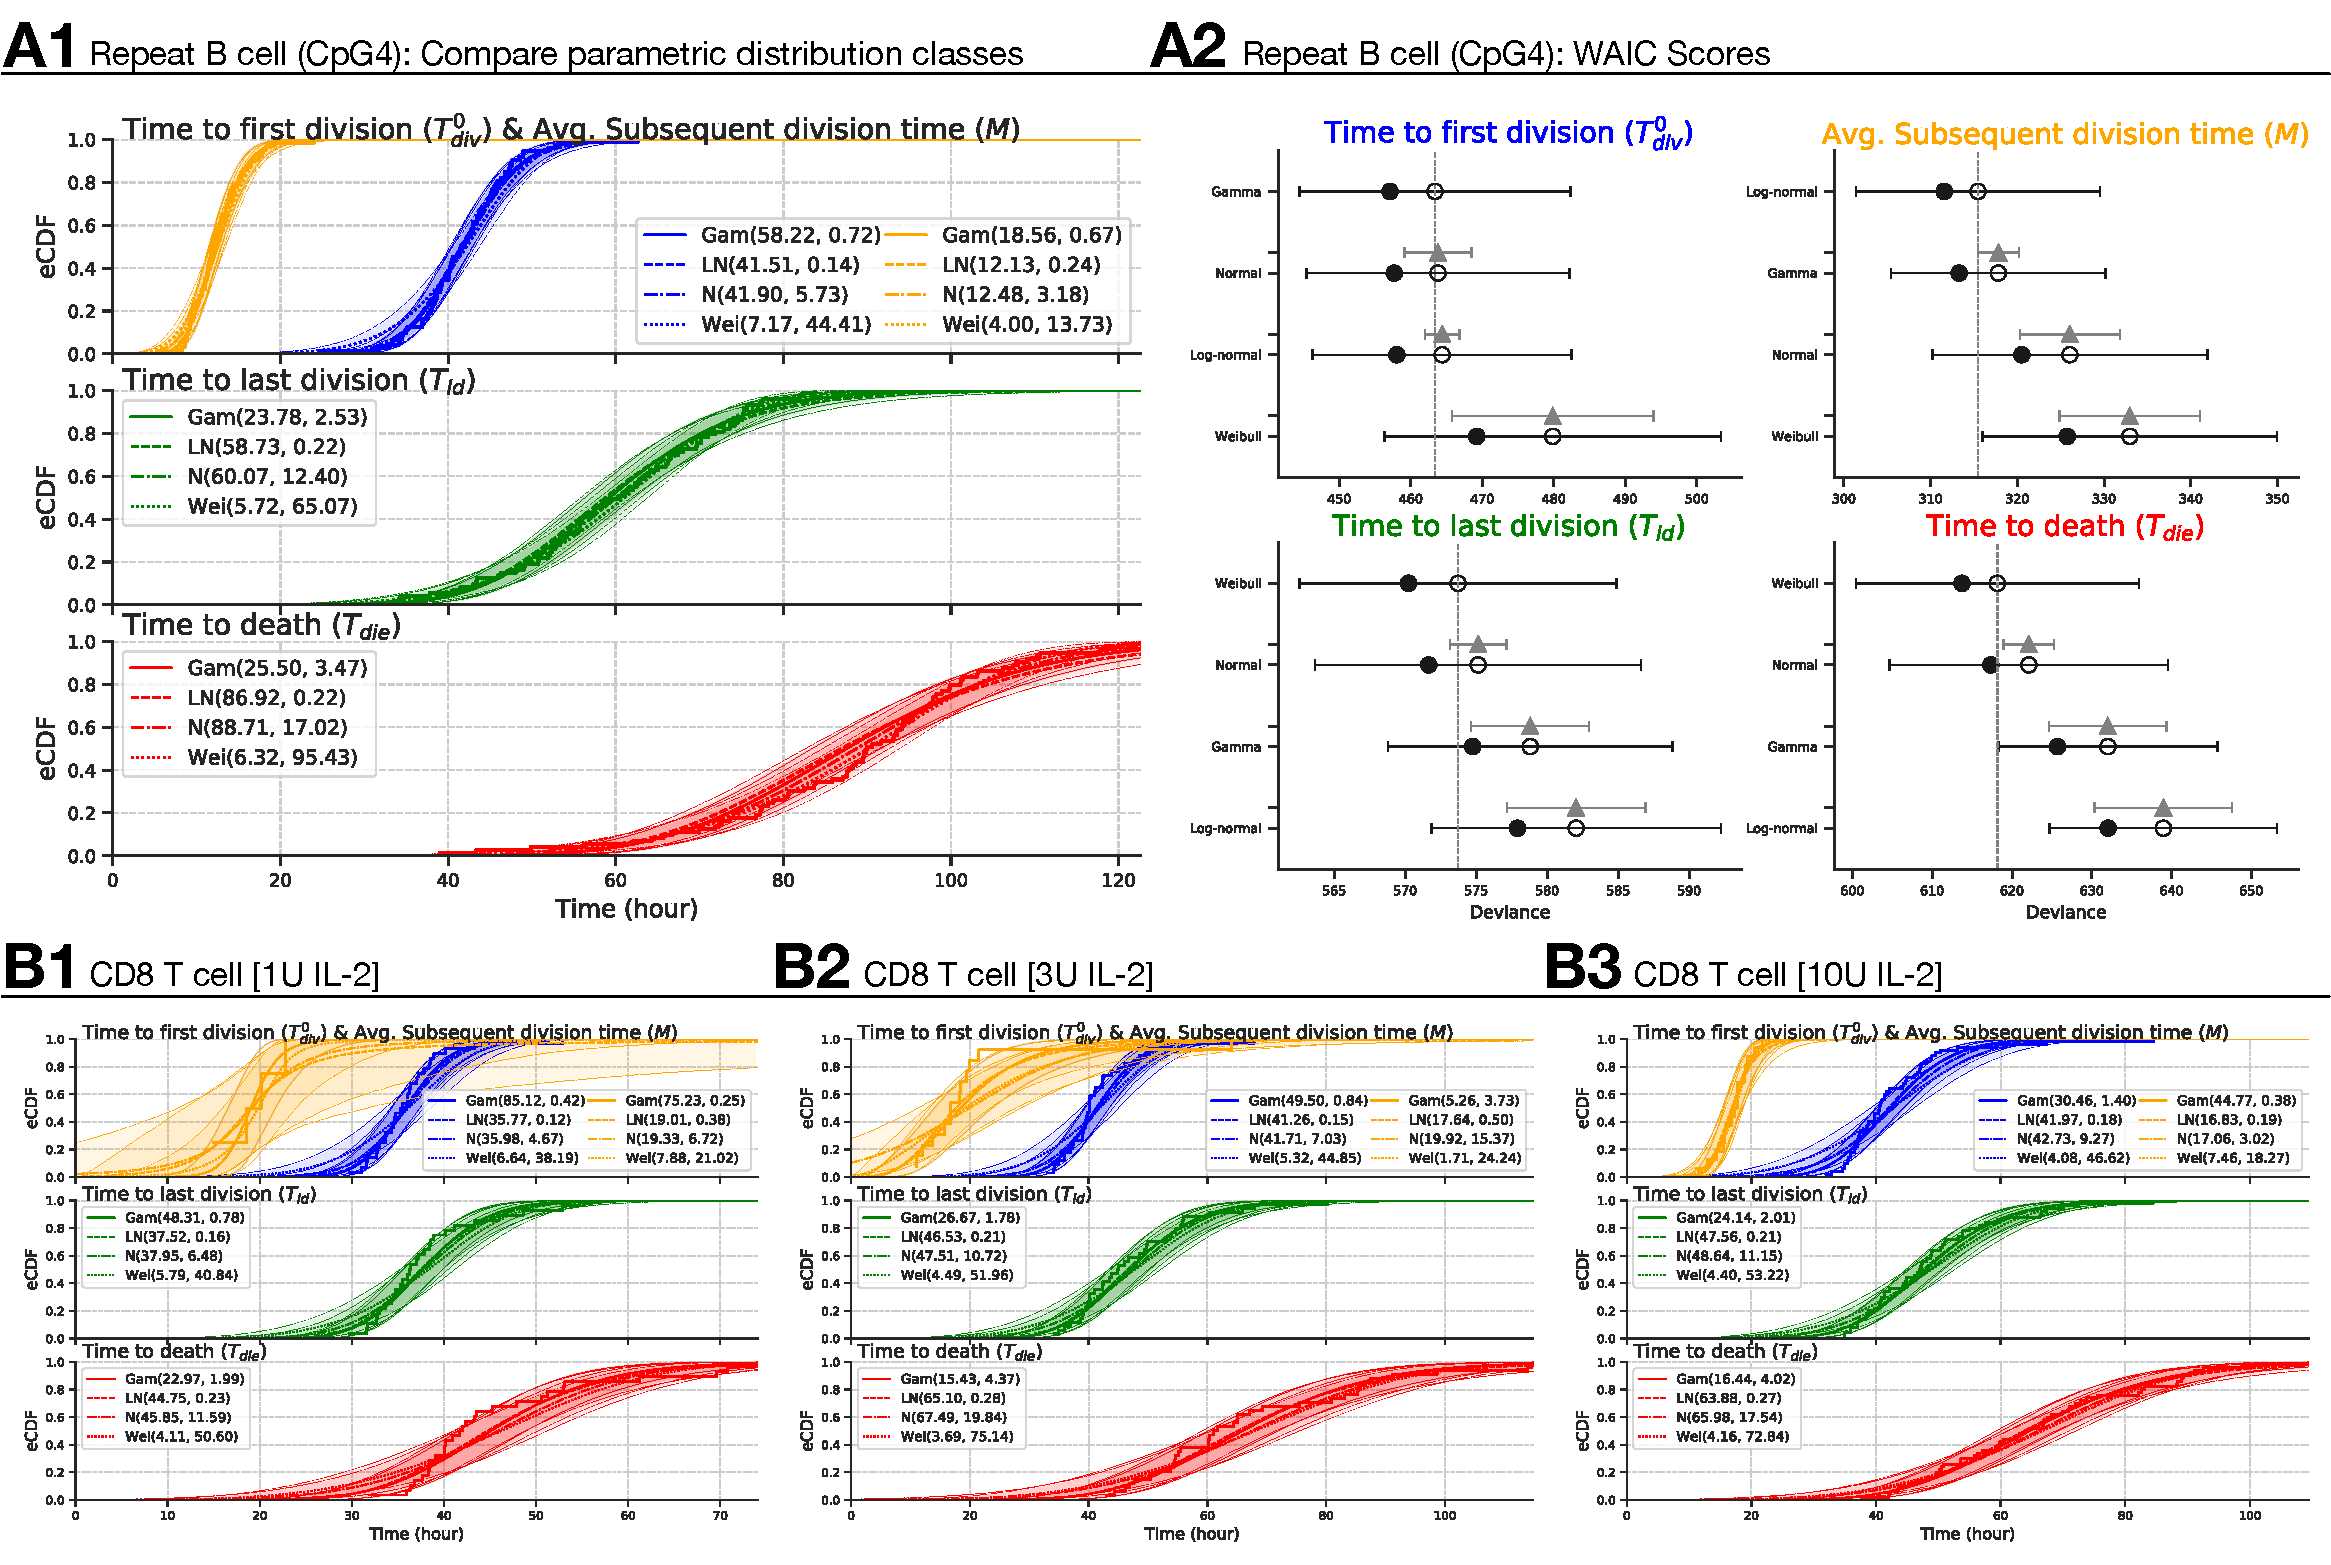
\includegraphics[scale=0.45]{figs/supp_fig4.pdf}
    \caption{\textbf{Best parametric distribution classes.} Four candidate distribution classes parameterised by: ($\alpha_G$, $\beta_G$) for Gamma; ($m$, $s$) median and scale for lognormal; ($\mu$, $\sigma$) mean and standard deviation for Normal; and, ($\alpha_W$, $\beta_W$) for Weibull. \textbf{(A1-2)} Repeat of CpG-stimulated B cell (CpG4). The solid line of CDF are plotted by taking the mean of each parameters in respective posterior distribution. \textbf{(B1-3)} CD8 T cell in the presence of 1U, 3U and 10U of IL-2. Corresponding distribution fits to the WAIC scores reported \cref{fig:best_distribution}B1-3 in the main text.}
    \label{supp_fig:best_distribution}
\end{figure}

\begin{figure}[h]
    \centering
    \includegraphics[scale=0.36]{figs/supp_fig5.pdf}
    \caption{\textbf{Best parametric distribution classes.} \textbf{(A1-4)} Experiment Costim1 consists of N4, N4+CD28, N4+IL2 and N4+CD28+IL2. \textbf{(B1-4)} Experiment Costim2 constists of N4, N4+CD28, N4+IL-12 and N4+CD28+IL12. Minimum of two observations per variable was required for the calculation.}
    \label{supp_fig:costim_best_distribution}
\end{figure}

\begin{figure}[h]
    \centering
    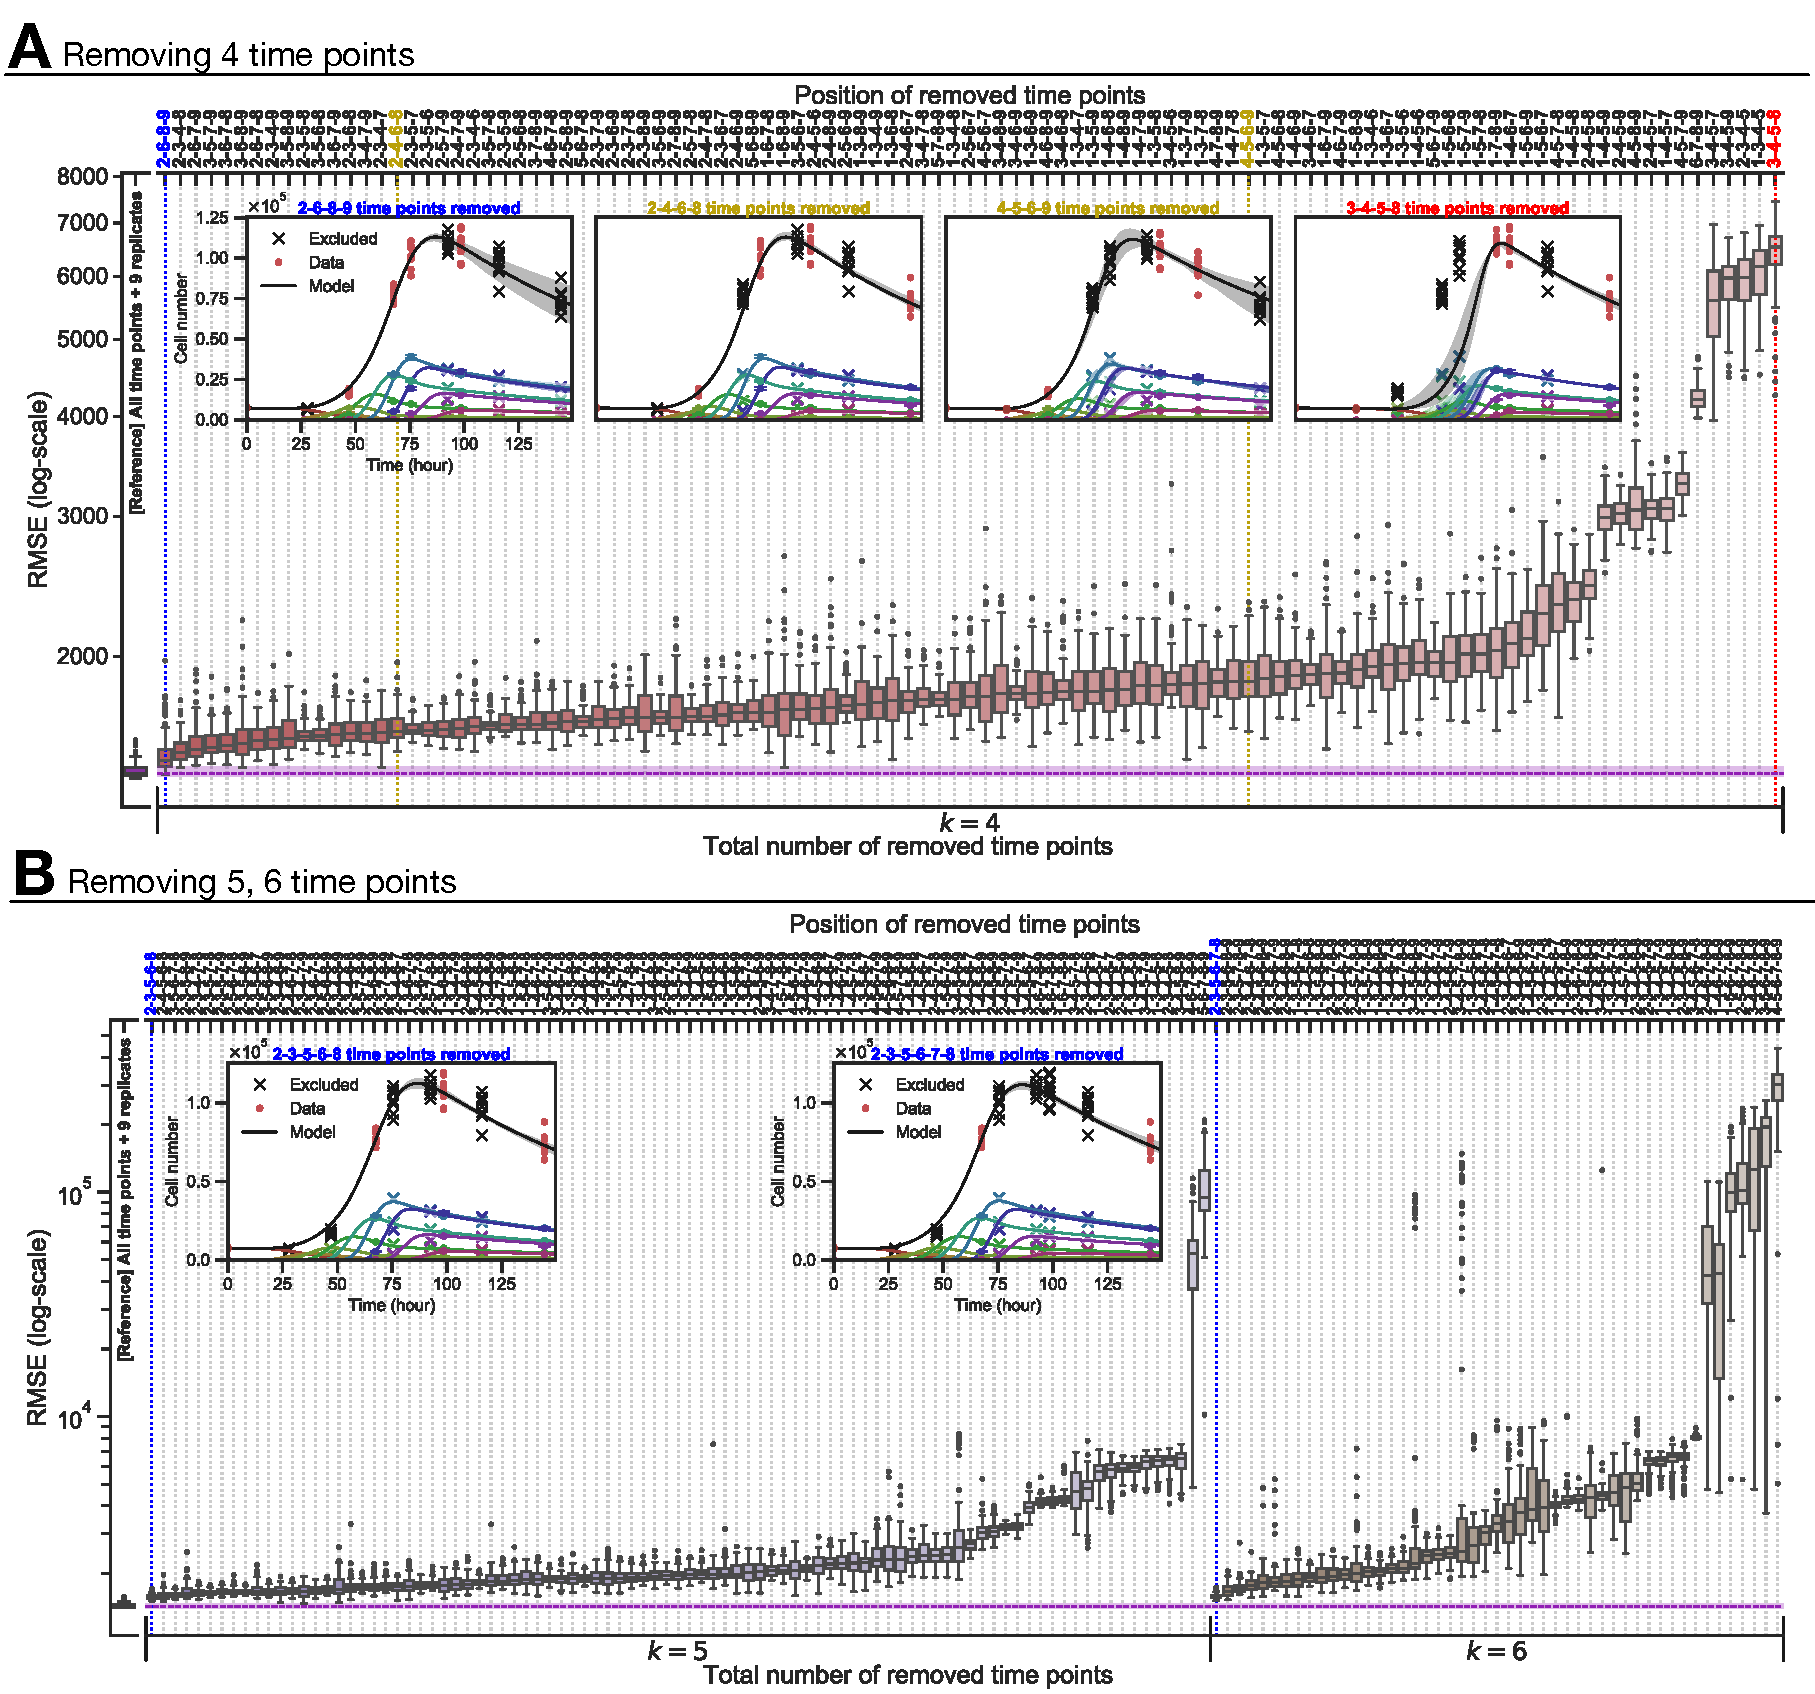
\includegraphics[scale=0.58]{figs/supp_fig6.pdf}
    \caption{\textbf{The accuracy of the model fit with CpG-stimulated Bim$^{-/-}$ B cell data.} Root-mean-squared error (RMSE) evaluated over all time points and replicates after fitting the Cyton2 model to artificially removed dataset. The reference RMSE (\textit{purple}) was obtained by fitting the model to all available data points. \textbf{(A)} All possible combinations of positions of time points for $k=4$ case. The best (\textit{blue}) and worse (\textit{red}) examples of Cyton fits are shown. \textbf{(B)} Best examples for $k=5,6$ are shown. The worst cases failed to provide good fits (not shown), resulting in large confidence bands and an order of magnitude difference in RMSE.}
    \label{supp_fig:removed_time_points}
\end{figure}

\begin{figure}[h]
    \centering
    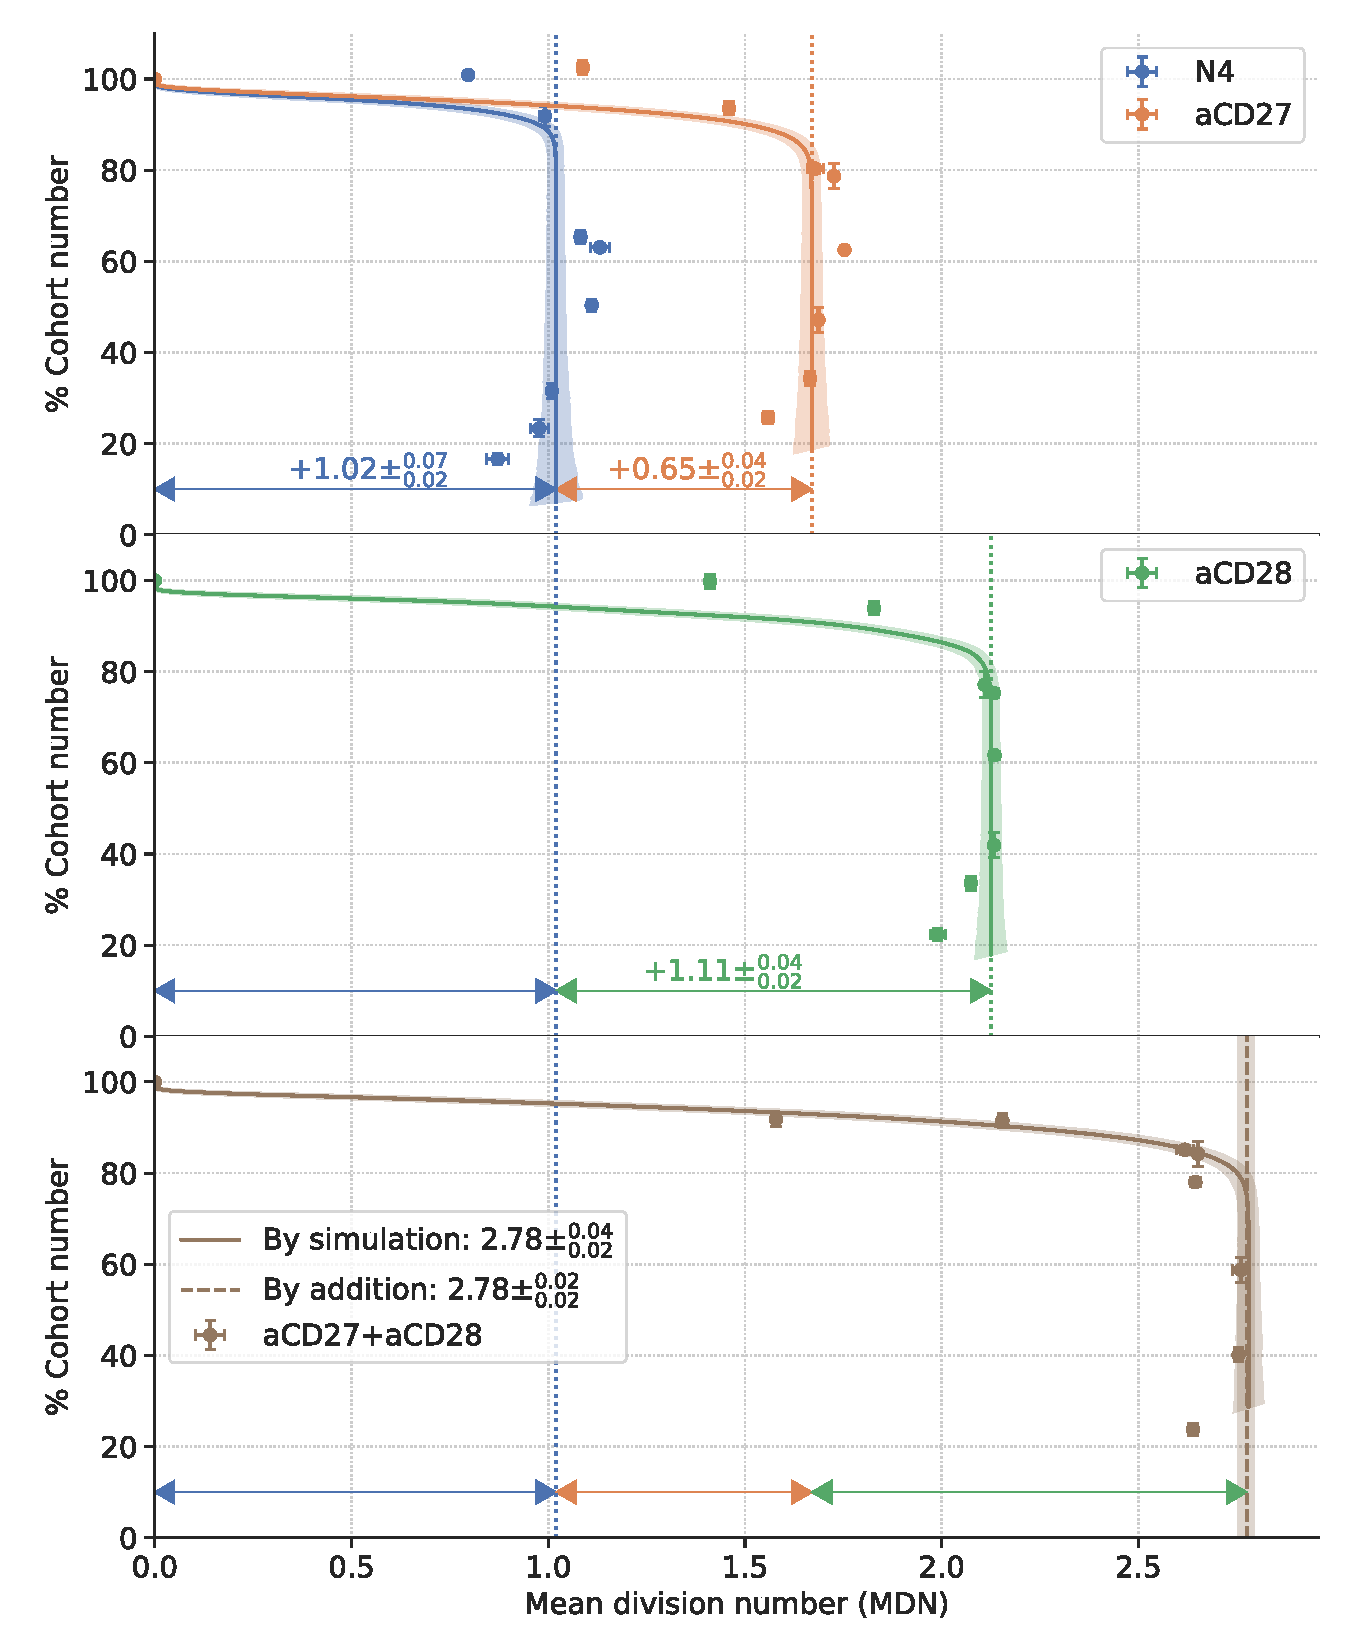
\includegraphics[scale=0.5]{figs/supp_fig7.pdf}
    \caption{\textbf{Linear sum of the signals from simulated trees \parencite{Marchingo.2014}.} The ABM was used to generate family trees. The times to fates were sampled from the estimated parameter values by fitting the Cyton2 model. To match the data ($\bullet$: mean $\pm$ SEM), each round of the simulation was initialised with 6066 (N4), 8252 (aCD27) and 8377 (aCD28) clones and ran for $t \in [0, 140]$ with $\Delta t = 0.5$ in hours. This process was repeated $10^3$ times to obtain 95\% confidence bands around the mean. Increase in MDN is labelled in each panel with arrows. The predicted MDNs for aCD27+aCD28 were calculated either by summing the contribution from each individual stimulation (\textcolor{brown}{\dashed}) or simulating the trees directly with the summed timers (\textcolor{brown}{\full}).}
    \label{supp_fig:recapitulate_application}
\end{figure}


\end{document}
